\renewcommand{\BrainFuckChapter}{y}
\renewcommand{\LifeChapter}{y}
\chapter{Background}
\label{chap:background}
\chaptertoc{}

\begin{chapterabstract}
  This chapter introduces the physics behind \ac{dMRI}, some techniques used for the simulation of \ac{dMRI} as well as some background on axonal growth mechanisms.
  Firstly, general MR physics is introduced building up from a single proton to the generation of the spin echo signal.
  The second section discusses how the diffusion of water molecules impacts the MR signal, leading to the diffusion signal attenuation.
  The third section introduces some simulation approaches which can be used to generate synthetic \ac{dMRI} data.
  The final section gives an overview of some of the mechanisms which drive axonal growth in nature and which for the inspiration for the synthetic growth algorithm presented in further chapters. 
\end{chapterabstract}

\section{MR Physics}
\label{sec:bg_mri_physics}
All forms of \emph{in vivo} use of magnetic resonance have their origins in the 1940s when Purcell, Torrey and Pound independently and almost simultaneously with Bloch, Hansen and Packard detected radio frequency signals from nuclei in ordinary matter\cite{Levitt2008, Barker2009,Bloch1946,Purcell1946}.
This discovery gave birth to the field of \ac{NMR} which has become widespread, with applications in a number of areas including chemistry, biology, materials science and medical imaging\cite{Barker2009, Salibi1998}.

Within the medical imaging context, \ac{NMR} typically finds two uses, \acf{MRI} and \ac{MRS}\footnote{The `N' from NMR is dropped in the medical imaging context to avoid confusion with nuclear medicine and general squeamishness around the word nuclear}.
Both of these uses are closely related: \ac{MRI} is typically concerned with building images of internal structures in the body, whilst \ac{MRS} is concerned with identifying the chemical composition of tissues in the body.

The theory behind \ac{NMR} concerns the interaction between nuclei and magnetic fields. This section briefly introduces the \ac{NMR} physics relevant to \ac{dMRI}.

\subsection{Nuclear Magnetism}
\label{sec:bg_nuclearmagnetism}

The most important property of a nucleus for the application of \ac{NMR} is nuclear spin. 
Spin is a property inherent to all subatomic particles and whilst it is a purely quantum effect, it can be thought of loosely as the particle spinning around its axis - much like a tiny planet \cite{Levitt2008}.
A planet spinning about its axis will have an angular momentum associated with that rotation and similarly the spin of a particle behaves like an angular momentum.
Unlike the angular momentum of a rotating planet, however, the spin is an intrinsic property of the particle itself and not a result of its motion\cite{Levitt2008}.

\begin{comment}
One of the postulates of quantum mechanics is that angular momentum is quantised \cite{DeGraaf2007}. This means that the spin angular momentum, $S$, of a particle in its rest state can only take values of
\begin{equation}
S = \hbar \sqrt{(I(I+1))} \,,
\label{eq:angmom_quant}
\end{equation} 
where $I$ is the spin angular momentum quantum number which can only take integer or half-integer values and $\hbar$ is the reduced Planck constant \cite{DeGraaf2007}.
A second quantum number is used to describe the direction of angular momentum relative to a given direction, usually referred to as $z$. 
Again, this quantum number is quantised, with the angular momentum in the $z$ direction, $S_z$, given by 
\begin{equation}
S_z = \hbar m_z \,.
\label{eq:angmom_z}
\end{equation} 
The $m_z$ quantum number can have $2I + 1$ values in the range \cite{DeGraaf2007}
\begin{equation}
m_z = -I,\, -I + 1,\,\dots,\, I-1,\, I\,.
\label{eq:m_z}
\end{equation}

Protons, neutrons and electrons - the particles making up all everyday matter - all have a spin quantum number of $I = \sfrac{1}{2}$ meaning that $m_z$ can have two possible values $m_z = \pm \sfrac{1}{2}$.


% \todo{IS THIS BIT NECESSARY? JUST FOCUS ON PROTONS?}
% Nuclei are made up of protons and neutrons, so the spin of a nucleus will be given by the combination of the spins of the protons and neutrons in the nucleus.
% In general in quantum mechanics, the combination of two angular momenta will result in a third angular momentum, which can take a range of values according to 
% \begin{equation}
% I_{12} = |I_1 - I_2|, |I_1-I_2| + 1, \dots, |I_1 + I_2| - 1, |I_1 + I_2|\,. 
% \end{equation}
 
% The precise way in which the spins combine in any given nucleus is a complicated quantum mechanical problem but there are some rules which describe the possible nuclear spin quantum numbers. 
% A nucleus with an odd mass number will have a half-integer spin, a nucleus with even mass number and even atomic number will have zero spin and a nucleus with an even mass number and odd atomic number will have integer spin \cite{DeGraaf2007}.

This project is focused on \ac{NMR} of \ce{^1H} nuclei in water molecules, which simply consist of a single proton and so have $I = \sfrac{1}{2}$. 
\ac{NMR} is, however, feasible on any nucleus with non-zero spin with some of the most biologically relevant nuclei for in-vivo MRS being \ce{^{13}C}, \ce{^{31}P} and \ce{^{23}Na} \cite{DeGraaf2007}.
\end{comment}


\ac{MRI} typically relies on \ac{NMR} of \ce{^1H} nuclei in water molecules, which simply consist of a single proton.
A proton carries a positive electric charge.
Just as classically a rotating charge with angular momentum, $\mathbf{L}$, will produce a magnetic moment, $
\boldsymbol{\mu} = \gamma \mathbf{L}$, the intrinsic spin angular momentum, $\mathbf{S}$ of a proton will produce a magnetic moment 
\begin{equation}
\label{eq:magnmom}
\boldsymbol{\mu} = \gamma \mathbf{S} \,,
\end{equation}
where $\gamma$ is the gyromagnetic ratio \cite{Levitt2008}.
For a proton, $\gamma = 2.675 \times 10^8$ rad s$^{-1}$ T$^{-1}$.

The fact that a proton has an intrinsic magnetic moment means that it will interact with magnetic fields and it is understanding this interaction that underpins \ac{NMR} theory.


\subsection{Magnetic Resonance}
\label{sec:bg_resonance}
Classically, a magnetic moment, $\boldsymbol{\mu}$, placed in an external magnetic field, $\mathbf{B}_0$, will feel a torque, $\boldsymbol{\tau}$, given by \cite{Haacke1999} 
\begin{equation}
\label{eq:torque}
\boldsymbol{\tau} = \boldsymbol{\mu} \times \mathbf{B}_0 \,.
\end{equation}
At the same time, classical mechanics gives a relationship between the change in angular momentum and the torque as \cite{Haacke1999} 
\begin{equation}
\label{eq:dLdt}
\frac{d\mathbf{L}}{dt} = \boldsymbol{\tau}\,. 
\end{equation}
For a proton in its rest state, the only angular momentum is the intrinsic spin angular momentum, $\mathbf{S}$, so combining \Cref{eq:torque,eq:dLdt} gives the equation of motion for a spin in an external magnetic field
\begin{equation}
\frac{d\mathbf{S}}{dt} = \boldsymbol{\mu} \times \mathbf{B}_0 \,.
\end{equation}
Since $\mathbf{S}$ is equivalent to $\boldsymbol{\mu}/\gamma$ (\Cref{eq:magnmom}), this becomes
\begin{equation}
\frac{d\boldsymbol{\mu}}{dt} = \gamma\boldsymbol{\mu} \times \mathbf{B}_0\,.
\label{eq:dmudt}
\end{equation}

This equation of motion can be solved in a few ways for the case of constant external magnetic field, with the result being that the magnetic moment precesses about the magnetic field with a frequency, $\omega_0$, given by\cite{Levitt2008}
\begin{equation}
\label{eq:LarmorFreq}
\omega_0 = \gamma B_0\,,
\end{equation}
with $B_0$ being the external field strength. 
This precessional motional is illustrated in \Cref{fig:precession}.
The frequency $\omega_0$ is known as the Larmor frequency and lies in the \ac{RF} range for typical field strengths found in MRI machines (1.5 - 7 T).

\begin{figure}
	\centering
	\begin{subfigure}{0.3\textwidth}
		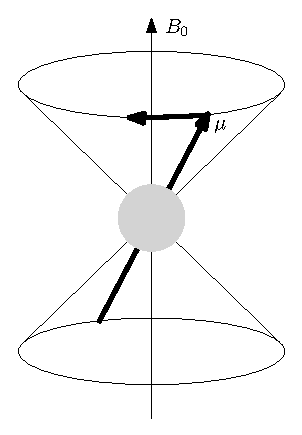
\includegraphics[width = \textwidth]{figures/background/precession.eps}
		\caption{}
		\label{fig:precession}
	\end{subfigure}
	\hspace{2cm}
	\begin{subfigure}{0.3\textwidth}
		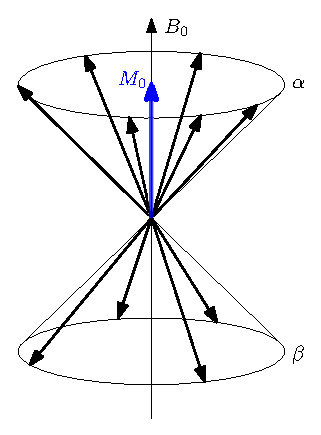
\includegraphics[width = \textwidth]{figures/background/manyspins.eps}
		\caption{}
		\label{fig:manyspins}
	\end{subfigure}
	
	\caption[Illustration of the precessional motion of a single spin and production of magnetisation by many spins]{a) Illustration of the precessional motion of a single spin with magnetic moment $\mu$ in the presence of an external magnetic field $B_0$. b) Many individual spins in an external magnetic field precess around the external field with random phase producing a net magnetisation in the direction of the $B_0$ field.}
	\label{fig:precession-spins}
	
\end{figure}


In practice, it is not possible to observe the magnetic moment of a single spin. 
The quantity observed is rather the sum of the magnetic moments from many spins together, this is known as the net magnetisation. 
%In order to fully describe the system, a quantum mechanical treatment using density operators is necessary \cite{Levitt2008}, however a classical treatment is sufficient to understand the basic principles.

\begin{comment}
As mentioned in \Cref{sec:bg_nuclearmagnetism}, protons can have two $S_z$ states with $m_z = \pm \sfrac{1}{2}$. 
These states can be thought of as the magnetic moment either being aligned parallel or anti-parallel to the external magnetic field, known as spin-up and spin-down respectively.

\begin{figure}
	\centering
	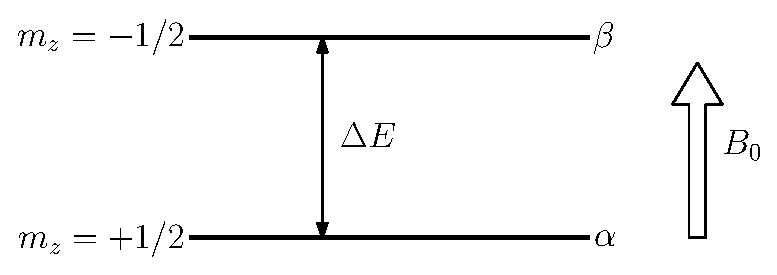
\includegraphics[width=0.6\textwidth]{figures/background/energy_levels.eps}
	\caption{Energy levels of a spin-1/2 particle. The spin-up state ($\alpha$) has the lowest energy and the spin down state ($\beta$) has the highest. The energy difference between the levels is $\Delta E$.}
	\label{fig:energylevels}
\end{figure}

The energy difference between these two states is given by a quantum mechanical effect called the Zeeman effect \cite{Levitt2008}, which gives the difference as  
\begin{equation}
	\Delta E = \gamma \hbar B_0\,.
\end{equation} 

\Cref{fig:energylevels} illustrates this splitting of the energy levels showing that the spin-up state, $\alpha$, is the lower of the two energy states. 
When there are many protons all experiencing the same magnetic field, the proportion of the number of protons in the spin-up, $n_\alpha$, state versus spin-down, $n_\beta$, is given by the Boltzmann distribution\cite{DeGraaf2007}
\begin{equation}
\frac{n_\alpha}{n_\beta} = \exp\left(\frac{\Delta E}{k_BT}\right)\,,
\end{equation}  
where $k_B$ is the Boltzmann constant and $T$ is the temperature. This means that at a non-zero temperature and with positive $\gamma$, there are slightly more protons aligned with the magnetic field than against it.  
\end{comment}


In a sample, slightly more protons will align with the $\mathbf{B}_0$ field than against it, meaning that the net magnetisation will be parallel to $\mathbf{B}_0$. 
\Cref{fig:manyspins} shows a pictorial representation of the system of many spins producing a net magnetisation, $\mathbf{M}_0$ aligned with $\mathbf{B}_0$.

Each of the spins will still be precessing about the magnetic field at the Larmor frequency but since they are out of phase with one another, all transverse components of the magnetisation cancel out when they combine and all that is left is a static longitudinal component. 


In order to make measurements, the net longitudinal magnetisation needs to be `flipped' into the transverse plane where it can be detected. 
This is achieved by applying a second magnetic field, $\mathbf{B}_1$, oscillating in the transverse plane. 
In much the same way as with $\mathbf{B}_0$, the magnetisation feels a torque from $\mathbf{B}_1$ and begins to rotate about $\mathbf{B}_1$, away from the longitudinal axis.
The two external fields act simultaneously on $\mathbf{M}_0$ so the magnetisation will tip away from the $z$ axis whilst still precessing about $z$ with a frequency $\omega_0$.
This kind of motion is known as nutation and is illustrated in \Cref{fig:nutation}.

\begin{figure}
	\centering
	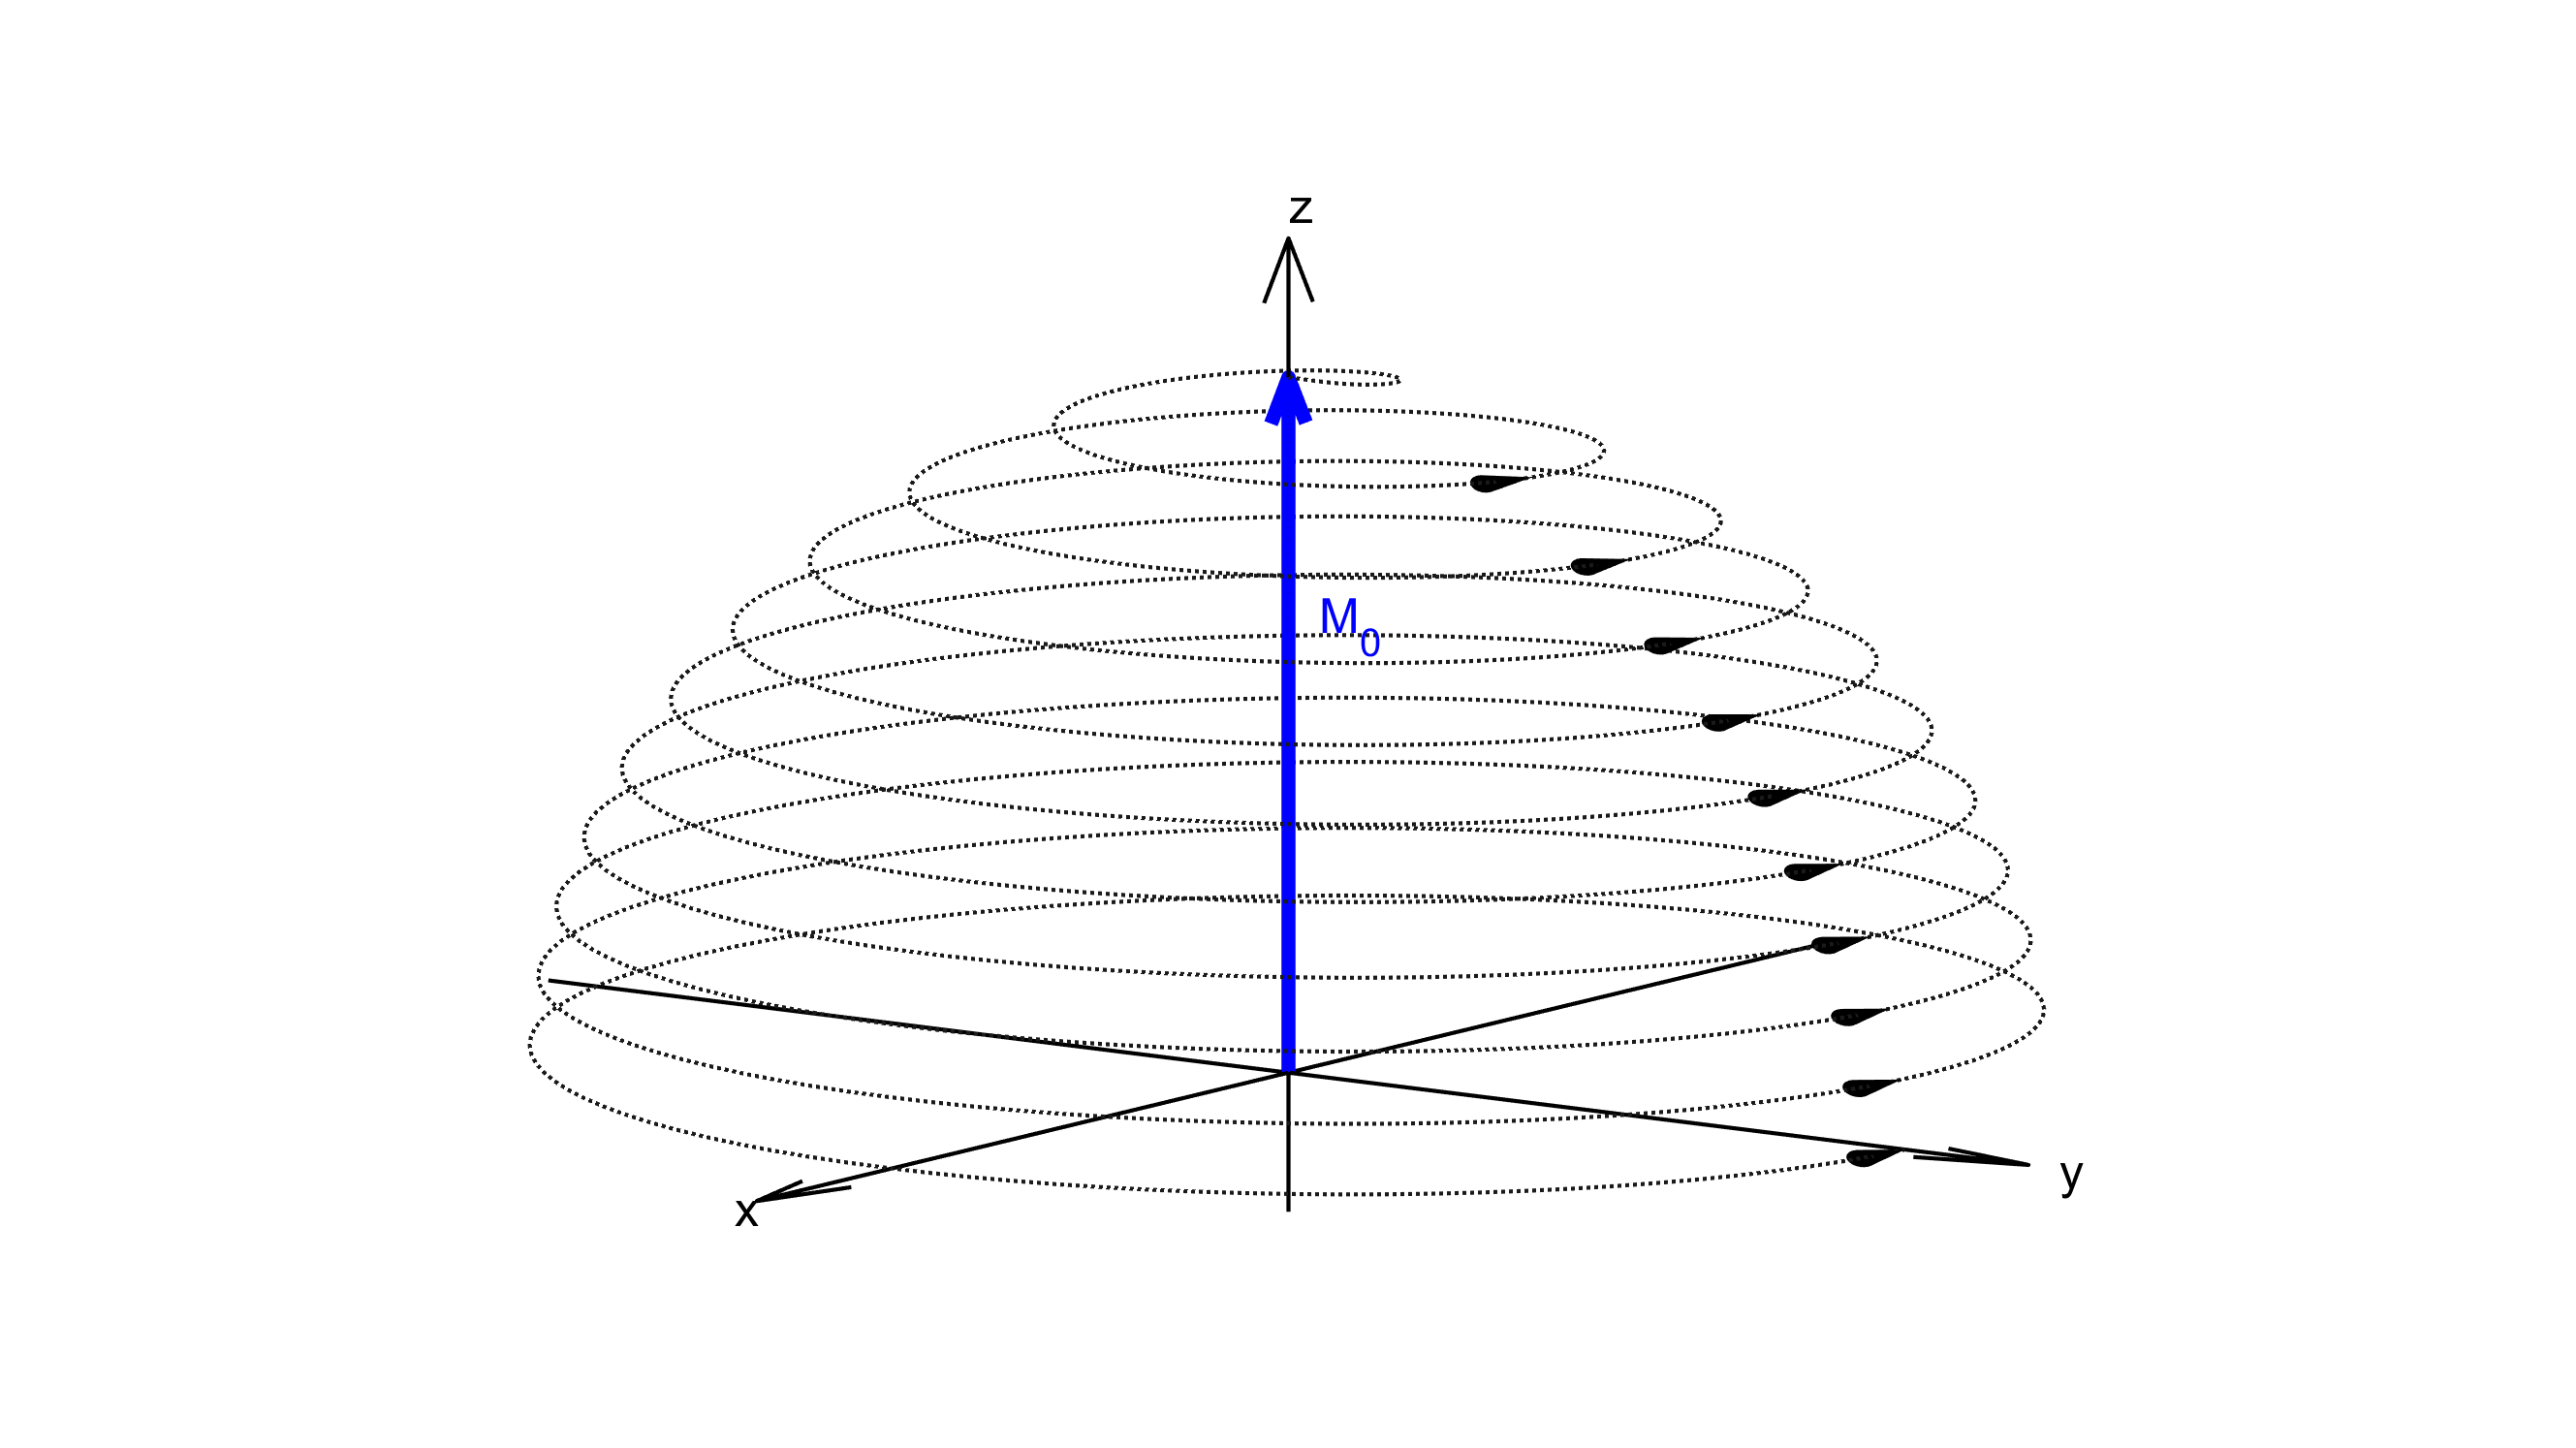
\includegraphics[width=\textwidth]{figures/background/nutation.eps}
	\caption[Nutation motion of an on-resonance spin the presence of an \ac{RF} field.]{Nutation motion of an on-resonance spin in the presence of an \ac{RF} field. Precession about the $B_0$ and $B_1$ fields create the spiralling motion in the laboratory frame.}
	\label{fig:nutation}
\end{figure}



\subsection{The Bloch Equations}
\label{sec:bg_bloch}
The interaction between the magnetisation and magnetic fields is described by the Bloch equations - an empirical set of equations describing the evolution of magnetisation introduced by Felix Bloch in 1946\cite{Bloch1946}.

The magnetisation arises from a sum of independent magnetic moments, meaning that we can represent the magnetisation as 
\begin{equation}
	\mathbf{M} = \sum_i \boldsymbol{\mu}_i \,,
        \label{eq:net_magnetisation}
\end{equation}
with $i$ indicating a sum over all the spins in the sample.
This definition for $\mathbf{M}$ can be combined with the equation of motion for a single spin, \Cref{eq:dmudt}, to give \cite{Haacke1999}
\begin{equation}
	\frac{d\mathbf{M}}{dt} = \gamma \mathbf{M} \times \mathbf{B}\,.
	\label{eq:dMdt}
\end{equation}  

In the presence of the main external field, $\mathbf{B}_0$, the magnetisation will be static and aligned along the $z$ axis. The $x$ and $y$ components of the magnetisation will have random orientations and precess about $\mathbf{B}_0$ at the Larmor frequency with a mean amplitude of zero. This will give the components of \Cref{eq:dMdt} as\cite{DeGraaf2007}
\begin{align}
	\frac{d\mathbf{M}_x(t)}{dt} &= \gamma\mathbf{M}_y\mathbf{B}_0\,,\\
	\frac{d\mathbf{M}_y(t)}{dt} &= -\gamma\mathbf{M}_x\mathbf{B}_0\,,\\	\frac{d\mathbf{M}_z(t)}{dt} &= 0 \,.
\end{align}

To understand the interaction of the magnetisation with the $\mathbf{B}_1$ field, the oscillation of the field in the transverse plane needs to be described. 
%The $\mathbf{B}_1$ field is oscillating in the transverse plane, say, along the $x$-axis. 
%The linearly oscillating field in $x$ can be thought of as two components rotating about the $z$-axis, one with a frequency $\omega$ and one with a frequency $-\omega$. 
%The sum of these two components will result in a field that is linearly oscillating along $x$ with a frequency $\omega$. \todo{Change/Mention that circularly polarised fields are used}
%
%Supposing that this frequency is on the same order as the Larmor frequency, one of the components (for a spin with positive $\gamma$ this will be the $+\omega$ component) will differ from the Larmor frequency by about $2\omega$. 
%This means that the effect of this component on the magnetisation can be neglected and the exciting magnetic field will have the form\cite{DeGraaf2007}
Usually, the $\mathbf{B}_1$ field is circularly polarised to oscillate in the transverse plane so that the field can be described as
\begin{equation}
	\mathbf{B}_1(t) = B_1\cos(\omega t) \mathbf{\hat{x}} - B_1\sin(\omega t) \mathbf{\hat{y}}\,,
	\label{eq:circB1}
\end{equation}
where $\mathbf{\hat{x}}$ and $\mathbf{\hat{y}}$ are unit vectors in the $x$ and $y$ directions respectively. 


The combined effect of the $\mathbf{B}_0$ and $\mathbf{B}_1$ fields can be seen from \Cref{eq:dMdt} to get \cite{DeGraaf2007}
\begin{align}
	\frac{d\mathbf{M}_x(t)}{dt} &= \gamma \left(\mathbf{M}_y(t)\mathbf{B}_0 - \mathbf{M}_z(t)\mathbf{B}_1\sin(\omega t)\right)\,,\label{eq:bloch_norelx}\\
	\frac{d\mathbf{M}_y(t)}{dt} &= \gamma \left(\mathbf{M}_z(t)\mathbf{B}_1\cos(\omega t) - \mathbf{M}_x(t)\mathbf{B}_0\right)\,,\label{eq:bloch_norely}\\
	\frac{d\mathbf{M}_z(t)}{dt} &= \gamma \left(\mathbf{M}_x(t)\mathbf{B}_1\sin(\omega t) - \mathbf{M}_y(t)\mathbf{B}_1\cos(\omega t) \right)\,.\label{eq:bloch_norelz}
\end{align}

These are the equations of motion of the magnetisation in the laboratory frame under the influence of the $\mathbf{B}_0$ and $\mathbf{B}_1$ and describe the kind of motion seen in \Cref{fig:nutation}. 

\subsubsection{Relaxation}
In order to get to the full Bloch Equations the concept of relaxation must be introduced. 
Relaxation is a term used to describe the way in which a spin system will return to equilibrium after being perturbed. The components of $\mathbf{M}$ that are parallel to the $\mathrm{B_0}$ magnetic field relax differently to those perpendicular to the magnetic field leading to two relaxation terms being introduced into \Cref{eq:bloch_norelx,eq:bloch_norely,eq:bloch_norelz}. 

The relaxation processes are exponential and described by two time constants, $\mathrm{T}_1$ and $\mathrm{T}_2$. $\mathrm{T}_1$ is the longitudinal relaxation time and describes the rate at which longitudinal magnetisation regrows after a perturbation. 
$\mathrm{T}_2$ is the transverse relaxation time and describes the rate at which transverse magnetisation decays after a perturbation. 
$\mathrm{T}_2$ is always shorter than $\mathrm{T}_1$ since all the effects which contribute to $\mathrm{T}_1$ also contribute to $\mathrm{T}_2$ relaxation, however $\mathrm{T}_2$ relaxation is also affected by the spins going out of phase with one another.
The relaxation process can be written as \cite{DeGraaf2007}
\begin{align}
	\frac{d\mathbf{M}_x(t)}{dt} &= -\frac{\mathbf{M}_x(t)}{\mathrm{T}_2}\,,\label{eq:bloch_rel1}\\
	\frac{d\mathbf{M}_y(t)}{dt} &= -\frac{\mathbf{M}_y(t)}{\mathrm{T}_2}\,,\label{eq:bloch_rel2}\\
	\frac{d\mathbf{M}_z(t)}{dt} &= -\frac{\mathbf{M}_z(t) - \mathbf{M}_0}{\mathrm{T}_1}\,.\label{eq:bloch_rel3}
\end{align}
		
Combining \Cref{eq:bloch_norelx,eq:bloch_norely,eq:bloch_norelz} and \Cref{eq:bloch_rel1,eq:bloch_rel2,eq:bloch_rel3} gives the full Bloch equations
\begin{align}
	\frac{d\mathbf{M}_x(t)}{dt} &= \gamma\left(\mathbf{M}_y(t)\mathbf{B}_0 - \mathbf{M}_z(t)\mathbf{B}_1\sin(\omega t)\right) - \frac{\mathbf{M}_x(t)}{\mathrm{T}_2}\,,\label{eq:bloch_labx}\\
	\frac{d\mathbf{M}_y(t)}{dt} &= \gamma\left(\mathbf{M}_z(t)\mathbf{B}_1\cos(\omega t) - \mathbf{M}_x(t)\mathbf{B}_0\right) - \frac{\mathbf{M}_y(t)}{\mathrm{T}_2}\,,\label{eq:bloch_laby}\\
	\frac{d\mathbf{M}_z(t)}{dt} &= \gamma \left(\mathbf{M}_x(t)\mathbf{B}_1\sin(\omega t) - \mathbf{M}_y(t)\mathbf{B}_1\cos(\omega t) \right) - \frac{\mathbf{M}_z(t) - \mathbf{M}_0}{\mathrm{T}_1}\,. \label{eq:bloch_labz}
\end{align}

$\mathrm{T}_2$ is used to refer to relaxation due to intrinsic spin-spin interactions which cause spins to accrue phase relative to one another and thus the magnitude of the net transverse magnetisation is reduced when taking the sum in \Cref{eq:net_magnetisation} .
Other effects can also contribute to the loss of transverse magnetisation, such as magnetic field inhomogeneities which can add to the $\mathrm{T}_2$ relaxation.
This is referred to as $\mathrm{T}_2^*$, with
\begin{equation}
  \frac{1}{\mathrm{T}_2^*} = \frac{1}{\mathrm{T}_2} + \frac{1}{\mathrm{T}_2'}\,,
  \label{eq:t2star}
\end{equation}
where $\mathrm{T}_2'$ is the relaxation time associated with these external sources and $\mathrm{T}_2$ is the intrinsic spin-spin relaxation time. The $\mathrm{T}_2'$ effect can be negated using special MR pulse sequences which will be covered in \Cref{sec:spin_echoes}, however the intrinsic $\mathrm{T}_2$ relaxation cannot be avoided.  


\subsubsection{The Rotating Frame}
To this point, everything has been described in a static Cartesian frame known as the laboratory frame. 
The lab frame is not the most convenient reference frame to analyse the \ac{NMR} experiment in, however.
Moving to a frame which is rotating about $\mathbf{B}_0$ (i.e.\ the $z$-axis) at a frequency $\omega$ matching the $\mathbf{B}_1$ field oscillation simplifies the maths of the system. 
The axes of this rotating frame will be referred to as $x', y'$ and $z'$. 

The components of the magnetisation in the rotating frame can be calculated from the lab frame components as \cite{DeGraaf2007}
\begin{align}
	\mathbf{M}_x' &= \mathbf{M}_x\cos(\omega t) - \mathbf{M}_y\sin(\omega t)\,,\\
	\mathbf{M}_y' &= \mathbf{M}_x\sin(\omega t) - \mathbf{M}_x\cos(\omega t)\,,\\
	\mathbf{M}_z' &= \mathbf{M}_z\,.
\end{align}

The rotating frame Bloch equations can be calculated by combining these rotating frame magnetisation components with the lab frame Bloch equations\cite{DeGraaf2007}
\begin{align}
	\frac{d\mathbf{M}_x'(t)}{dt} &= \Omega\mathbf{M}_y'(t) - \frac{\mathbf{M}_x'(t)}{\mathrm{T}_2}\,,\label{eq:blochx}\\
	\frac{d\mathbf{M}_y'(t)}{dt} &= -\Omega\mathbf{M}_x'(t) + \gamma\mathbf{B}_1\mathbf{M}_z'(t) - \frac{\mathbf{M}_y'(t)}{\mathrm{T}_2}\,,\label{eq:blochy}\\
	\frac{d\mathbf{M}_z'(t)}{dt} &= -\gamma\mathbf{B}_1\mathbf{M}_y'(t) - \frac{\mathbf{M}_z'(t) - \mathbf{M}_0}{\mathrm{T}_1}\,,\label{eq:blochz}
\end{align} 
where $\Omega = \omega_0 - \omega$ is the offset frequency between the $\mathbf{B}_1$ field frequency and the Larmor frequency. 

Since the frame is rotating with a frequency $\omega$, the $\mathbf{B}_1$ field appears static in the rotating frame. 
The precessional motion that is seen in the lab frame ($\omega_0 = \gamma\mathbf{B}_0$) is reduced to a frequency $\Omega$ in the rotating frame. 
When $\Omega = 0$, meaning that $\mathbf{B}_1$ oscillates at the Larmor frequency, the magnetisation simply precesses about the $\mathbf{B}_1$ field towards the transverse plane as illustrated in \Cref{fig:onres}. 

\begin{figure}
	\centering
	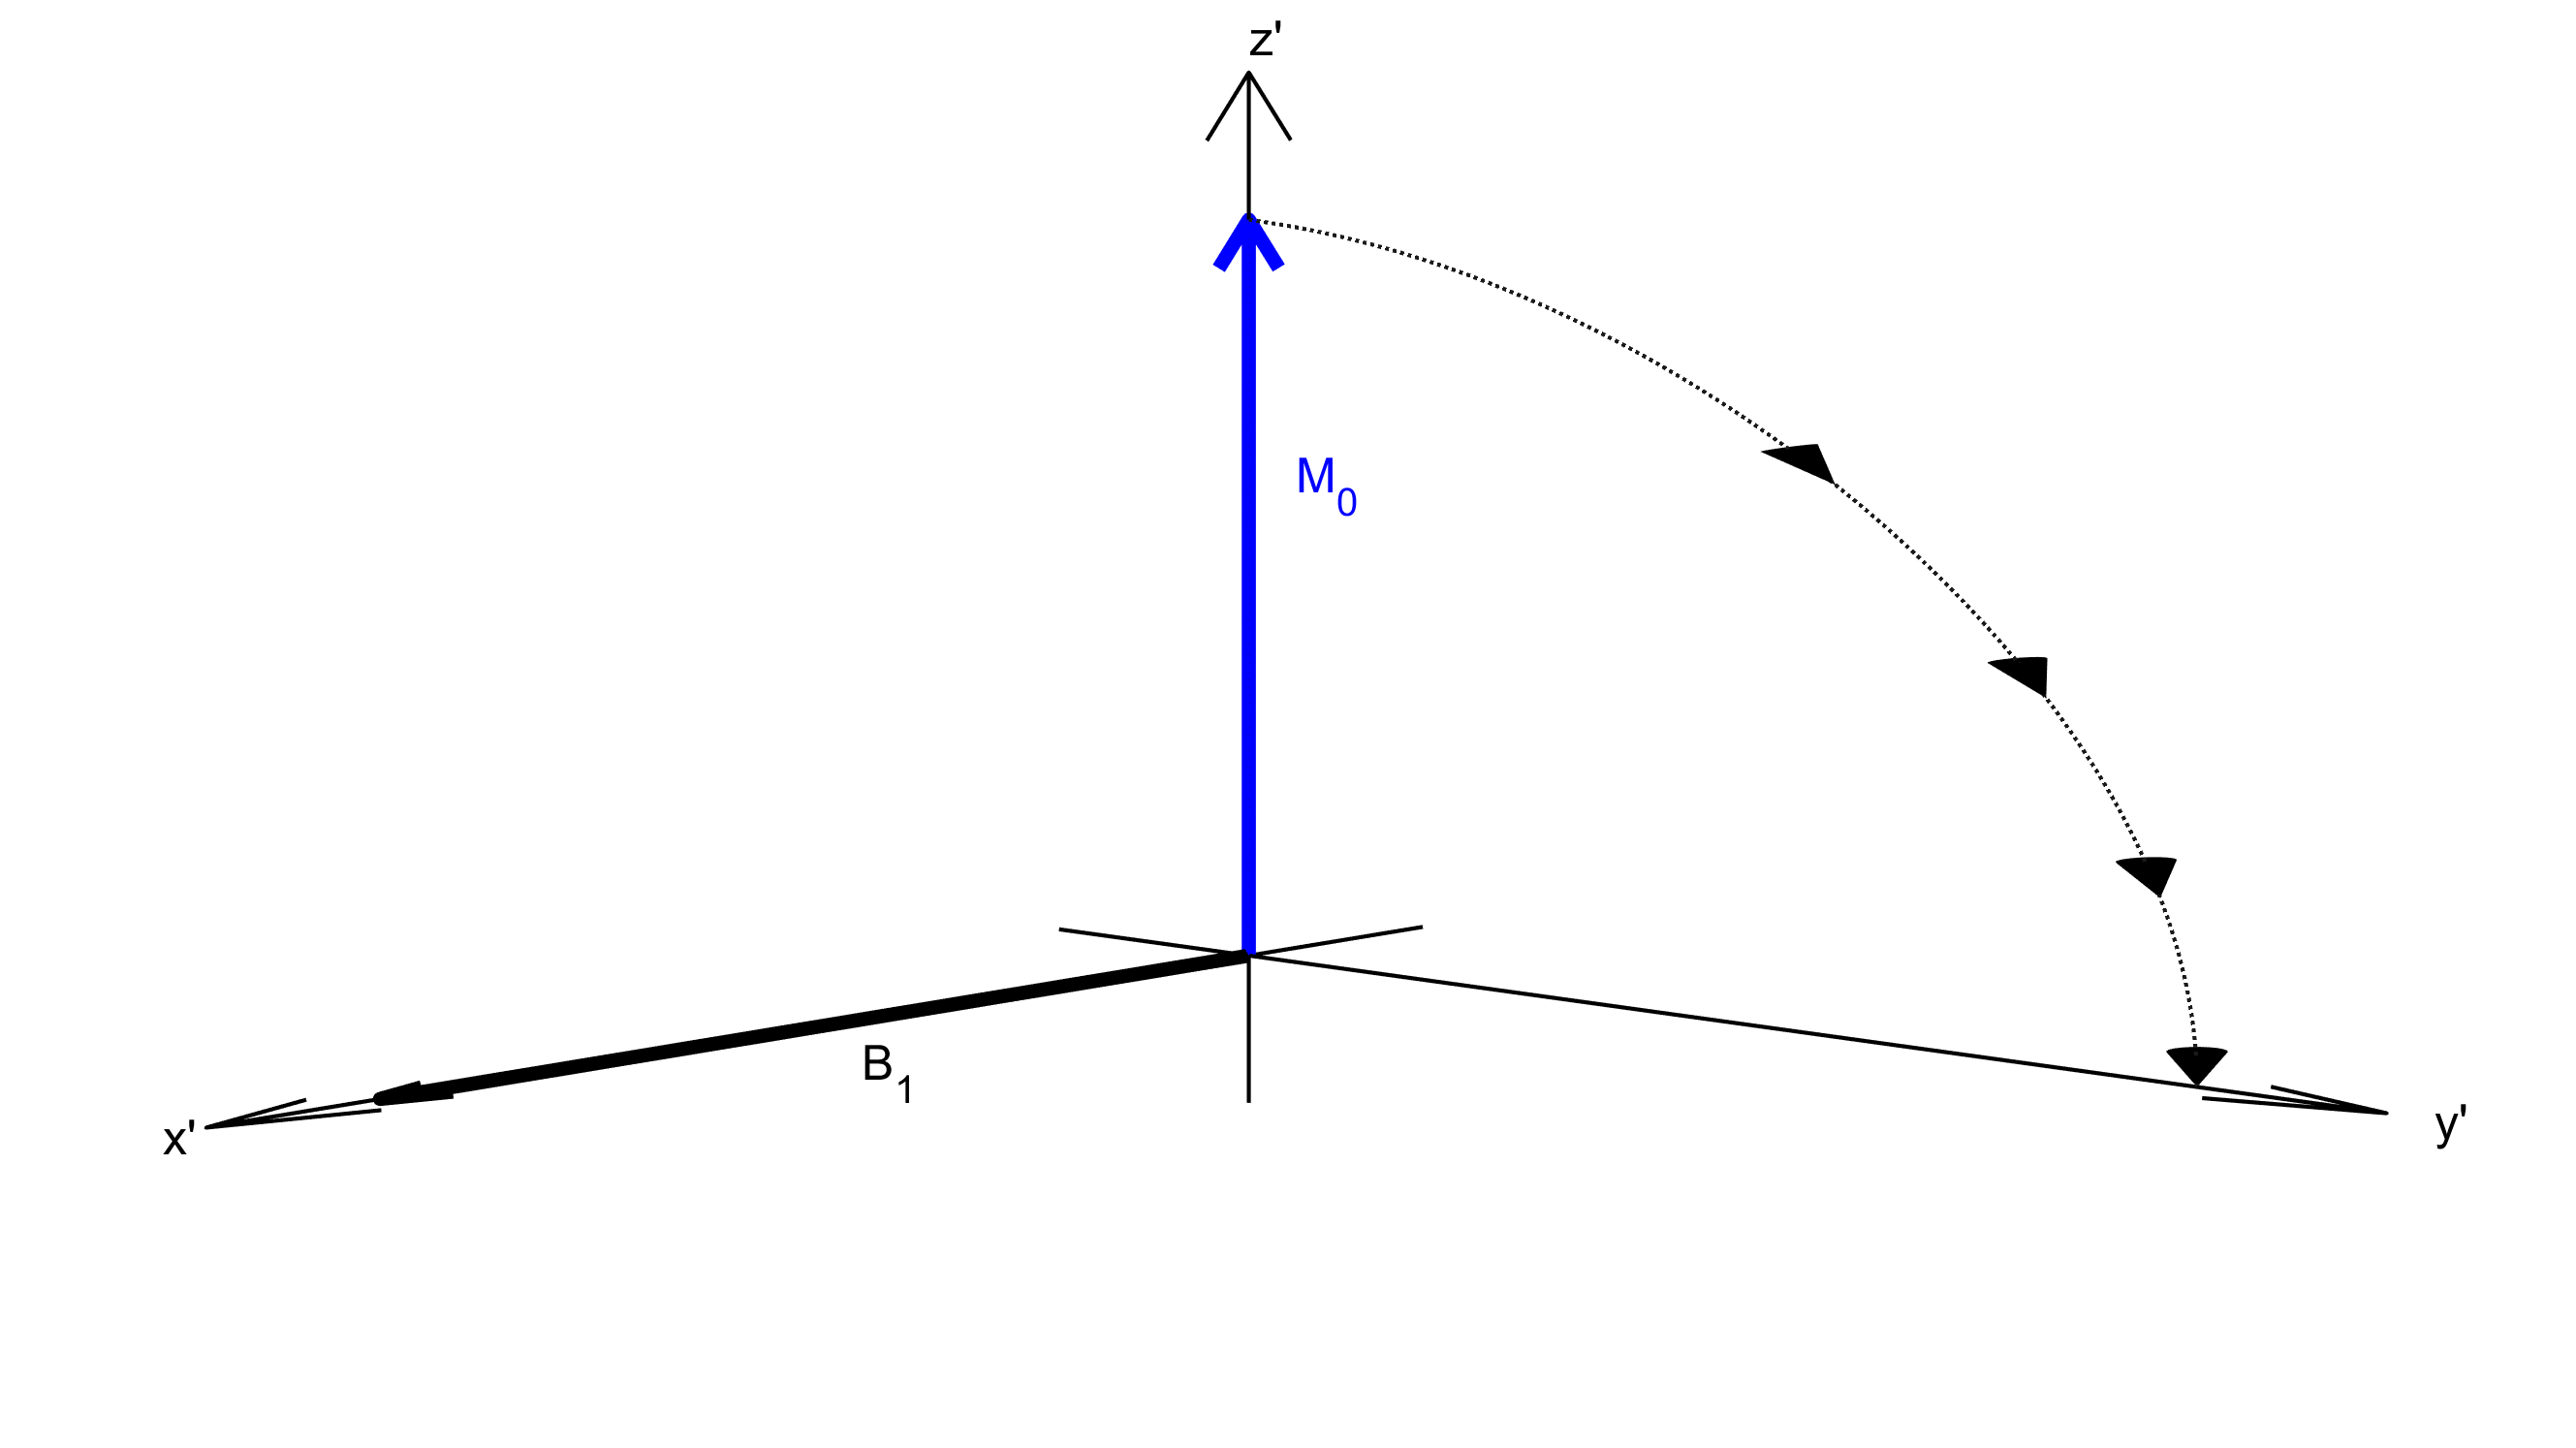
\includegraphics[width=\textwidth]{figures/background/nutation_onres.eps}
	\caption[Motion of a spin in the presence of a $B_1$ \ac{RF} field in the rotating frame]{Motion of a spin in the presence of a $B_1$ RF field in the rotating frame. This is identical to the nutation in \Cref{fig:nutation}, however viewing from the rotating frame simplifies the motion. }
	\label{fig:onres}
\end{figure}

This situation is known as resonance - the frequency of the \ac{RF} pulse matches the Larmor frequency, perfectly tipping the magnetisation away from the $z'$ axis and into the transverse plane. 

In the off-resonance case, an additional component of magnetic field with magnitude $\Omega/\gamma$ is produced in the $z$-direction.
This results in an effective magnetic field, $\mathbf{B}_e$, with a magnitude \cite{DeGraaf2007}
\begin{equation}
	B_e = |B_e| = \sqrt{B_1^2 + \left(\frac{\Omega}{\gamma}\right)^2}\,.
	\label{eq:Beff}
\end{equation}

%\todo[inline]{Do I need this off-resonance stuff? It's more geared towards introducing chemical shift for MRS. Perhaps just focus on signal generation?}
The effective field is illustrated in \Cref{fig:B_e} with the additional component of $\Omega/\gamma$ resulting in an effective field that is no longer aligned with $x'$.
\begin{figure}
	\centering
	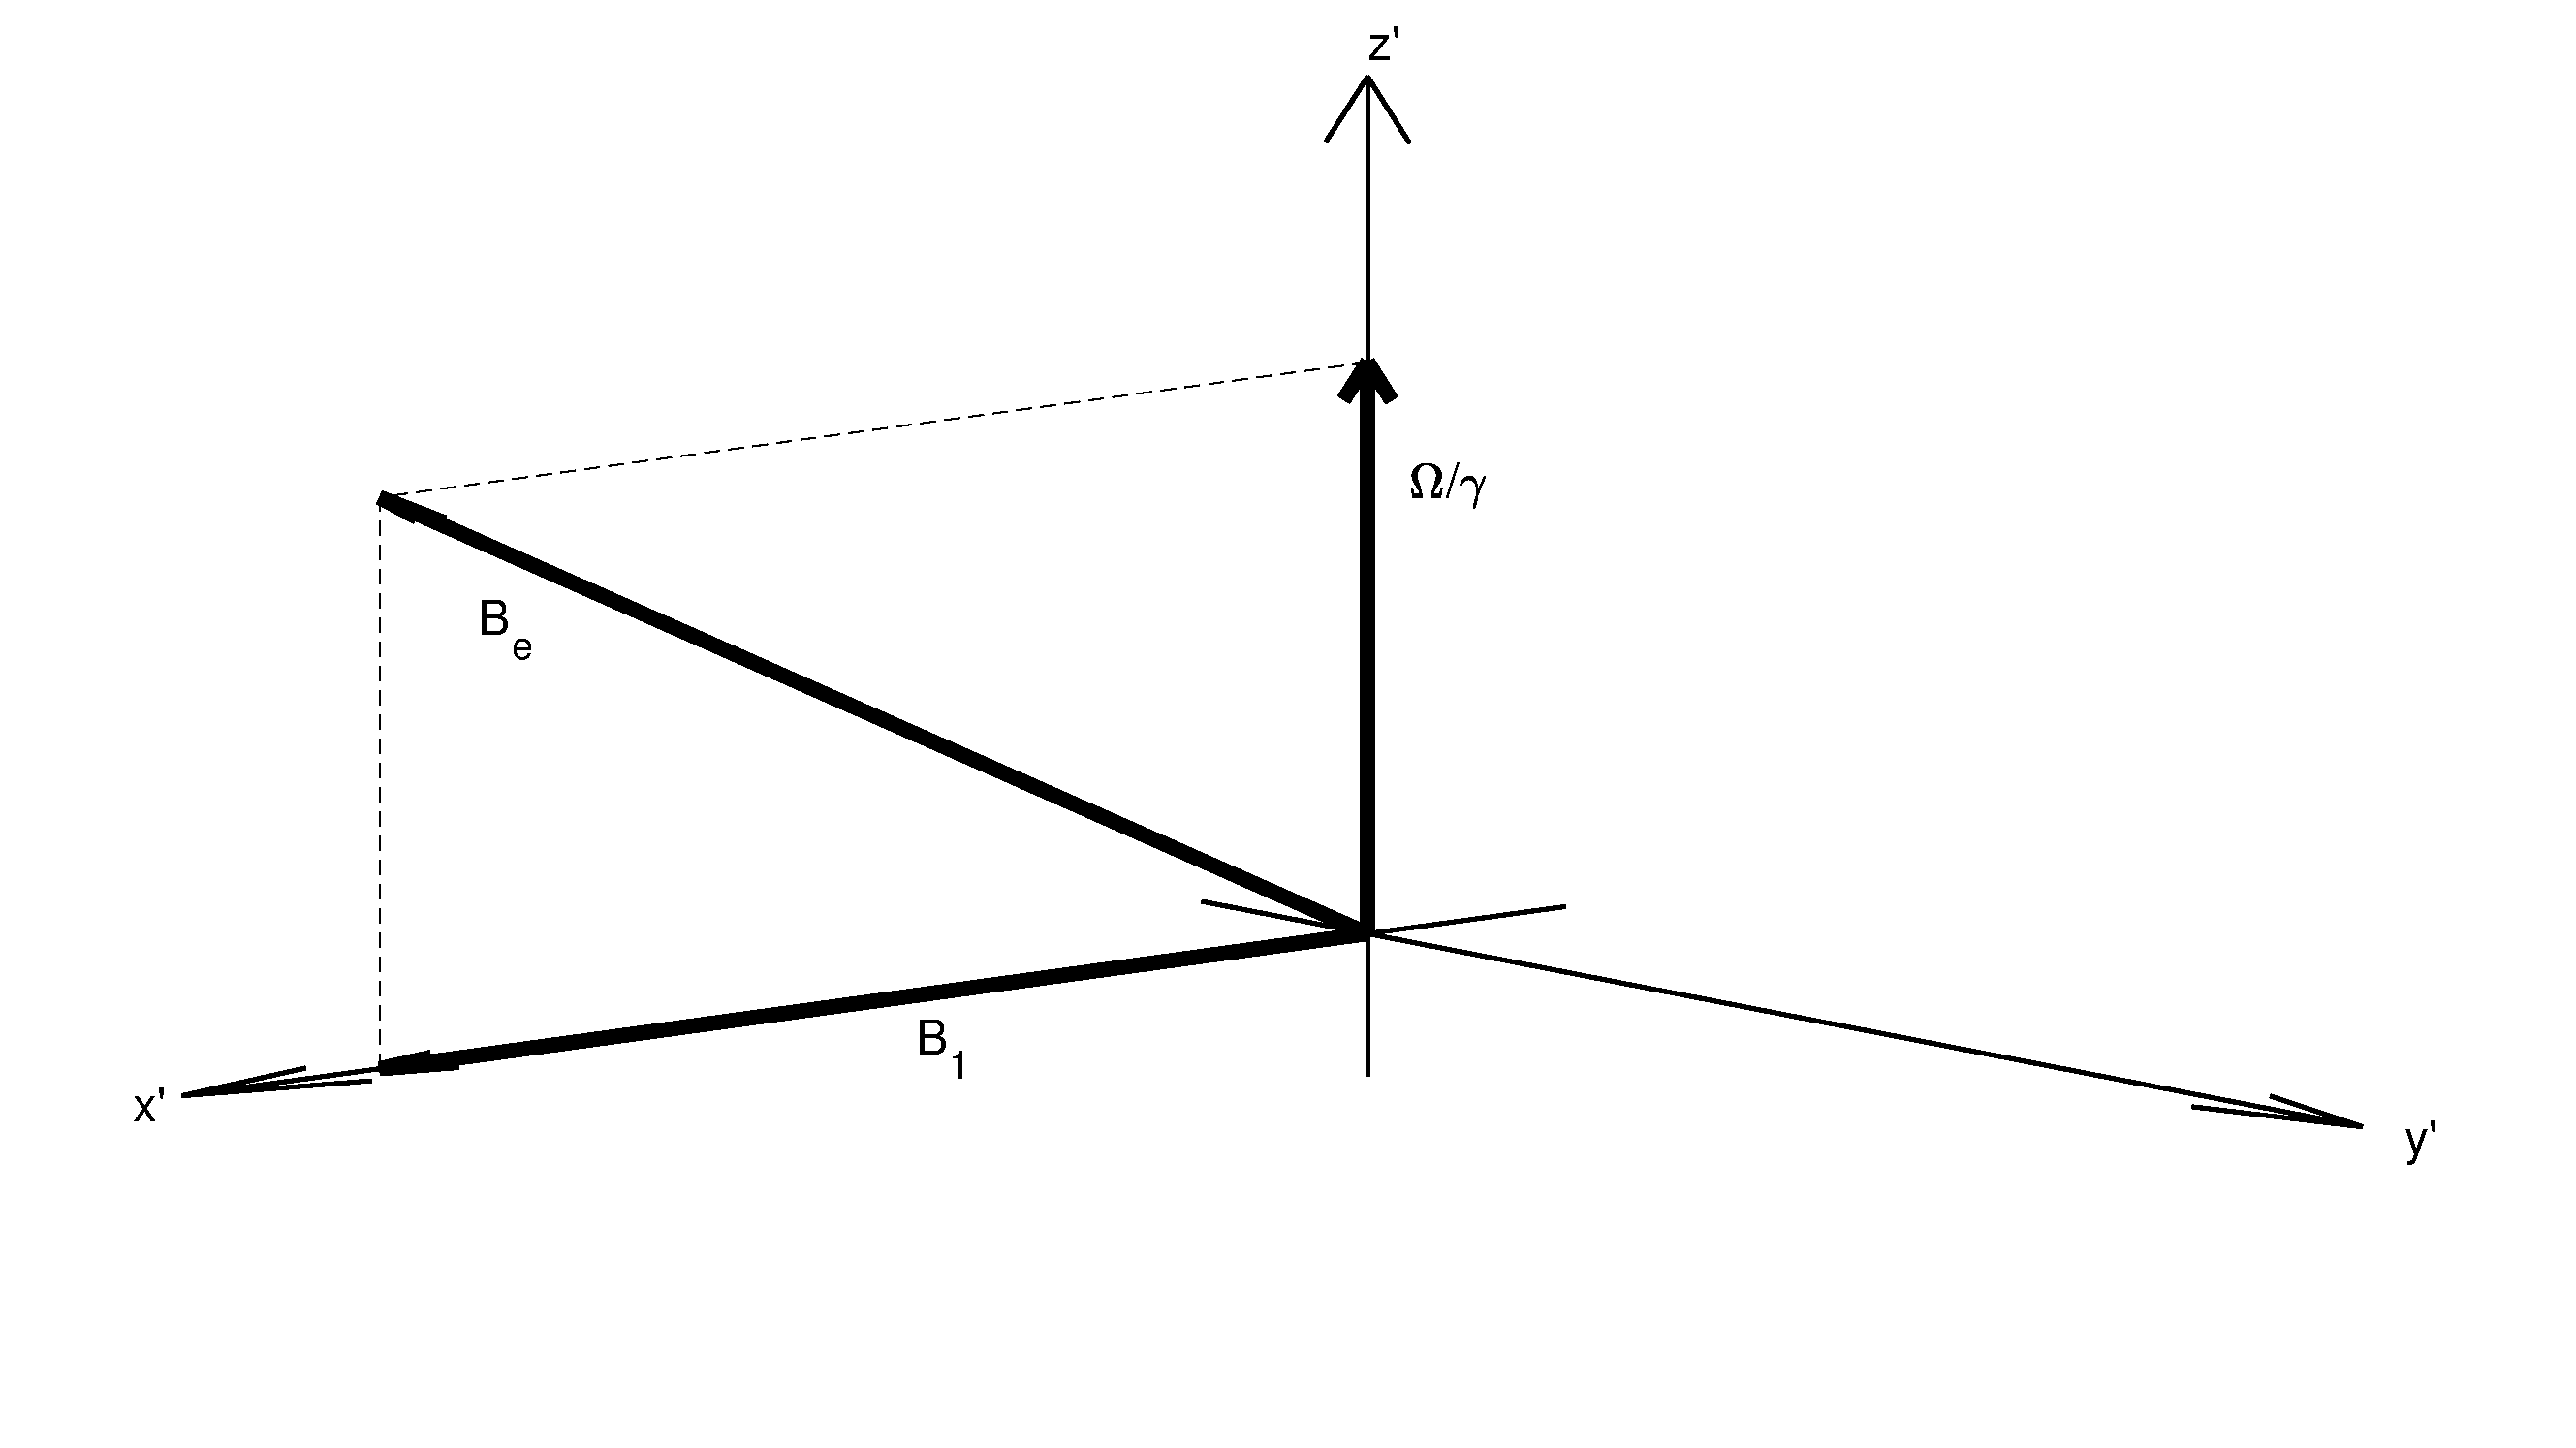
\includegraphics[width=\textwidth]{figures/background/B_e.eps}
	\caption[The effective field, $B_e$, produced due to an off-resonance frequency $\Omega$.] {The effective field, $B_e$, produced due to an off-resonance frequency $\Omega$. The off-resonance effects produce an additional component of magnetic field along the $z'$ axis.}
	\label{fig:B_e}	
\end{figure}
Off-resonance effects can produce unwanted results meaning the spin does not get flipped as much as expected under an \ac{RF} pulse which can result in signal losses. 
 

\subsection{Detecting the MR Signal}
The detection and processing of \ac{NMR} signals is a deep topic which could be the subject of its own book, however some very basic details of how a signal is formed are useful to go on from here.
 
The reason for flipping the magnetisation into the transverse plane using $\mathbf{B}_1$ fields is to make the magnetisation detectable. 
Transverse magnetisation precesses about $\mathbf{B}_0$ at the Larmor frequency, sweeping its magnetic field around $\mathbf{B}_0$. 
A coil of wire placed near this precessing field will feel an electromotive force induced in it according to Faraday's Law of Induction\cite{Haacke1999}.

Following a pulse that flips the magnetisation from $\mathbf{M}_0$ aligned with $z$ through an angle $\beta$ towards $x'$, the $x'$-component of the magnetisation will be $M_0\sin\beta$ and (ignoring relaxation) will then precess at the offset frequency, $\Omega$, in the rotating frame. This will give the components of the magnetisation in the transverse plane over time as 
\begin{equation}
M_x = M_0\sin(\beta)\cos(\Omega t) \qquad M_y = M_0\sin(\beta)\sin(\Omega t)\,.\label{eq:MxMy}
\end{equation}

The signal induced into the receiver coils is proportional to $M_x$ and $M_y$ and so the signal will also have an oscillating form similar to \Cref{eq:MxMy}.
From the $\sin\beta$ term, it is clear that the maximum signal will arise when $\beta = 90$\degree, meaning all the magnetisation is flipped into the transverse plane. 
Additionally, in a realistic experiment, there will be $\mathrm{T_2^*}$ relaxation so including this, the general form of the signal following a 90\degree\ pulse will be\cite{DeGraaf2007} 
\begin{equation}
S_x = S_0\cos(\Omega t)\exp\left(-t/\mathrm{T}_2^*\right) \qquad S_y = S_0\sin(\Omega t)\exp\left(-t/\mathrm{T}_2^*\right)\,.
\end{equation}

Generally \ac{NMR} systems use something known as quadrature detection, meaning that both the $x'$ and $y'$ components of the magnetisation are measured simultaneously\cite{Levitt2008}, giving the signal as a function of time as 
\begin{align}
	S(t) &= S_x + iS_y\,,\nonumber\\
		 &= S_0\exp((i\Omega - 1/\mathrm{T}_2^*)t)\,.\label{eq:fid}
\end{align}  

\begin{figure}
  \centering
  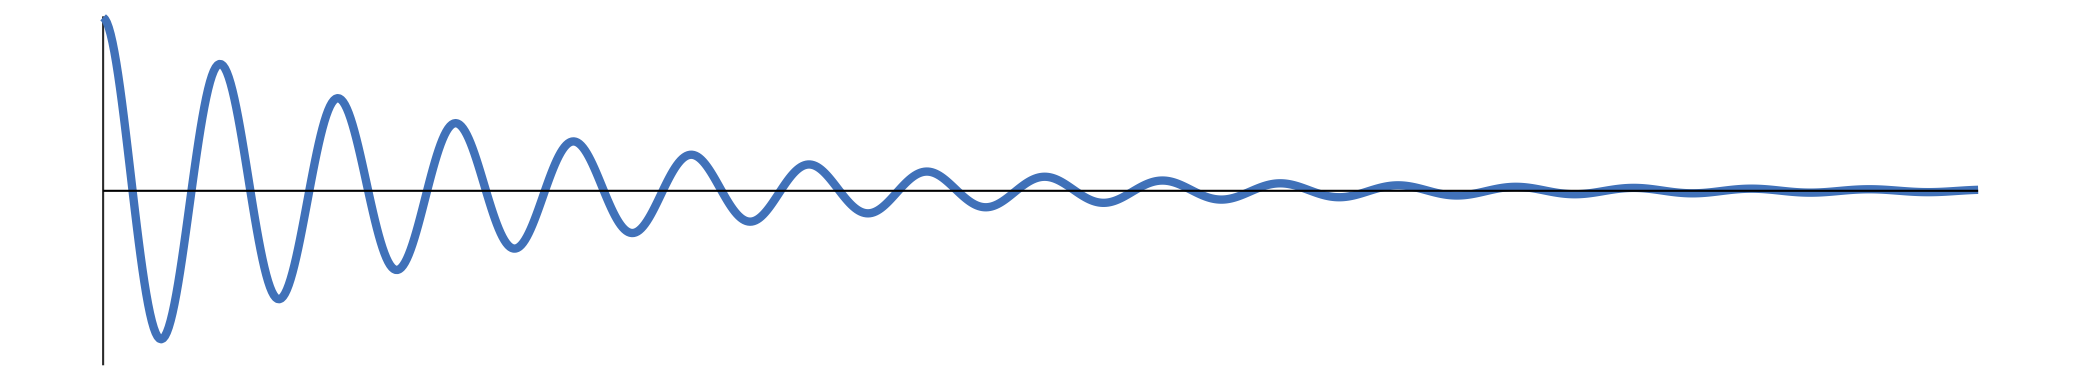
\includegraphics[width=\textwidth]{figures/background/FID_copy.png}
  \caption[The \acl{FID} described by \Cref{eq:fid}]{The \acl{FID} described by \Cref{eq:fid}. Here, just the real channel is plotted.}
  \label{fig:fid}
\end{figure}

This time-domain signal is known as a \ac{FID} and has a typical form shown in \Cref{fig:fid}. 
If we neglect off-resonance effects, then the \ac{FID} in the rotating frame will be a simple exponential decay.
\begin{equation}
  S(t) = S_0\exp(-t/\mathrm{T}_2^*)
  \label{eq:fid_rotframe}
\end{equation}

The \ac{FID} is not commonly used for \ac{dMRI} for a few reasons. Firstly, magnetic field gradients need to be introduced to make the signal sensitive to diffusion. Additionally, the $\mathbf{T}_2^*$ decay is often very rapid, so sequences known as spin echo sequences are used to remove the $\mathbf{T}_2'$ relaxation. 

\begin{comment}
The \ac{FID} holds all of the relevant information about the spin system needed for \ac{NMR}, however it is seldom used on its own since the information is difficult to interpret in this form.
\ac{NMR} spectroscopy uses a mathematical procedure known as the Fourier transform which is used as a transformation between the time and frequency domains. 
\begin{figure}
	\centering
	\begin{subfigure}{\textwidth}
		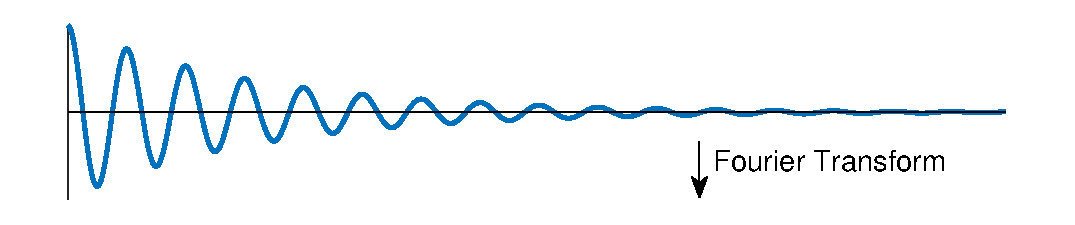
\includegraphics[width=\textwidth]{figures/background/FID.eps}
	\end{subfigure}

	\begin{subfigure}{\textwidth}
		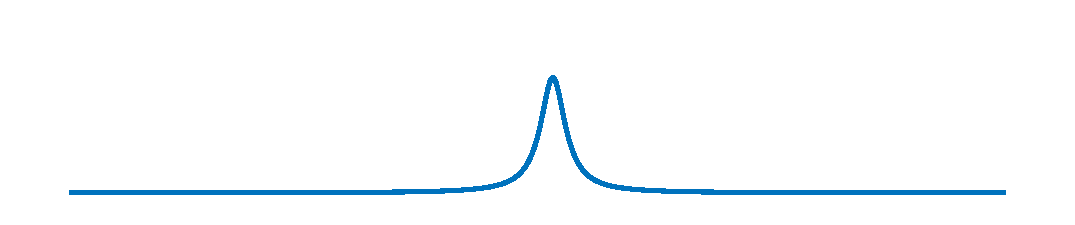
\includegraphics[width=\textwidth]{figures/background/fftFID.eps}
	\end{subfigure}
	\caption{An example of the Fourier transform. The time domain signal (top) is transformed into a frequency domain (bottom) by the Fourier transform. }
	\label{fig:fft}

      \end{figure}
      
Many books cover the Fourier transform in great detail \cite{Keeler2010, Haacke1999}, however for this report, it is sufficient to simply know its results.
The Fourier transform will take an \ac{FID} signal of the form in \Cref{eq:fid} and produce a frequency domain signal that has a mathematical form known as a Lorentzian, given by 
\begin{equation}
	S_0\exp((i\Omega - R_2)t) \quad\overset{\mathrm{FT}}{\rightarrow}\quad \frac{S_0R_2}{R_2^2 + (\omega - \Omega)^2} + i\frac{S_0(\omega - \Omega)}{R_2^2 + (\omega - \Omega)^2}\,,
\end{equation}    
where $\omega$ is the frequency domain of the spectrum. 
The real part of this term is known as the absorption mode and the imaginary part is known as the dispersion mode.
The absorption mode Lorentzian is shown in the bottom plot in \Cref{fig:fft}. 
Peaks like this form the basis of all spectra used in \ac{NMR} spectroscopy. 
\end{comment}



\subsection{Spin Echoes}
\label{sec:spin_echoes}
\begin{figure}
	\centering
	\begin{subfigure}{0.9\textwidth}
		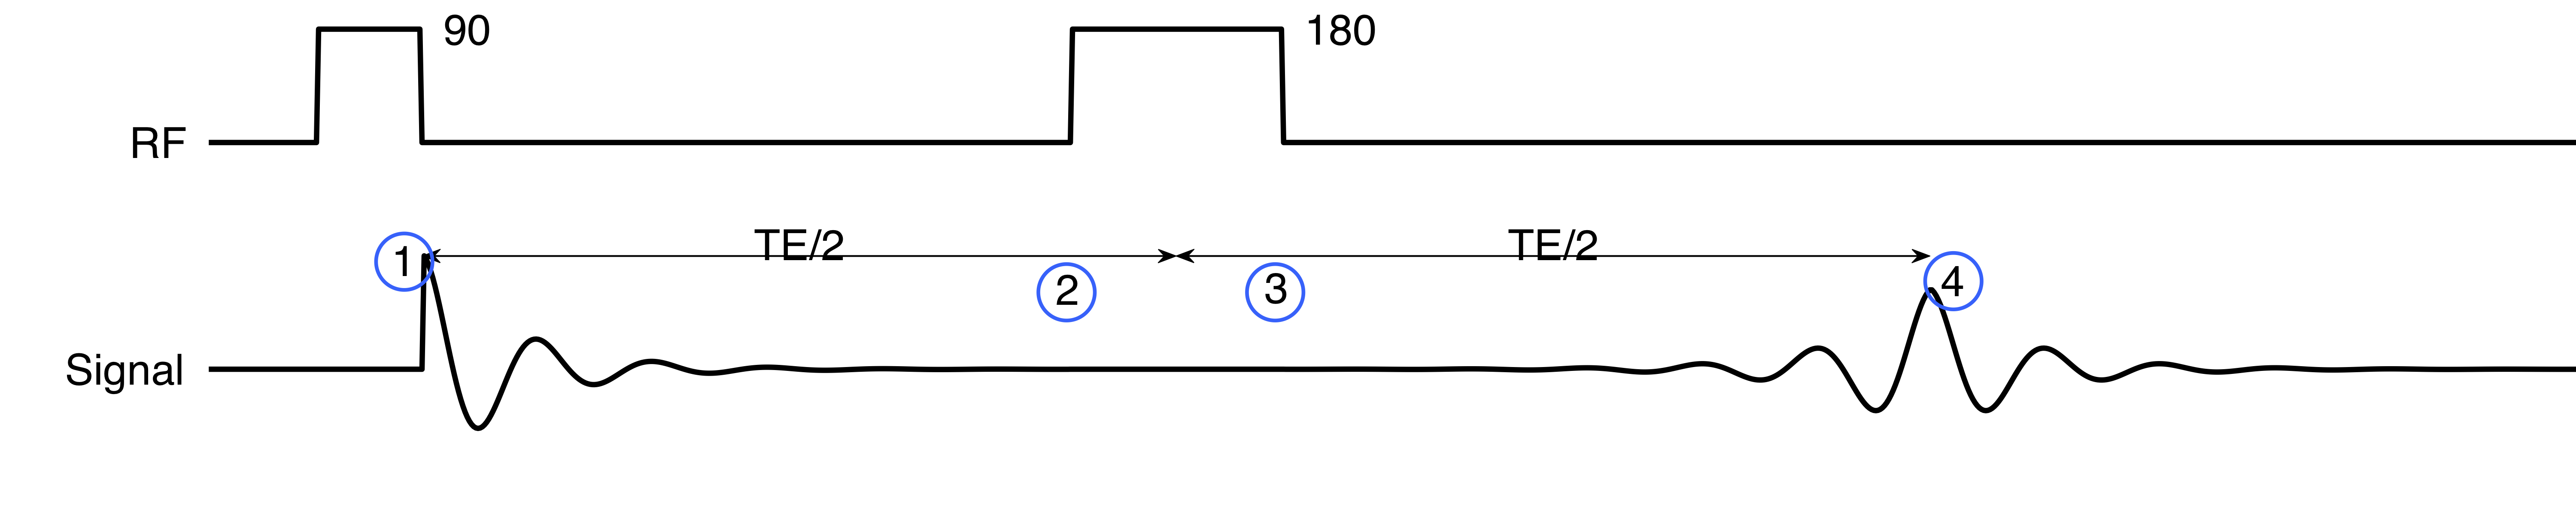
\includegraphics[width = \textwidth]{figures/background/spinecho.png}
		\caption{}
		\label{fig:spinechosequence}
	\end{subfigure}
	
	\begin{subfigure}{0.9\textwidth}
		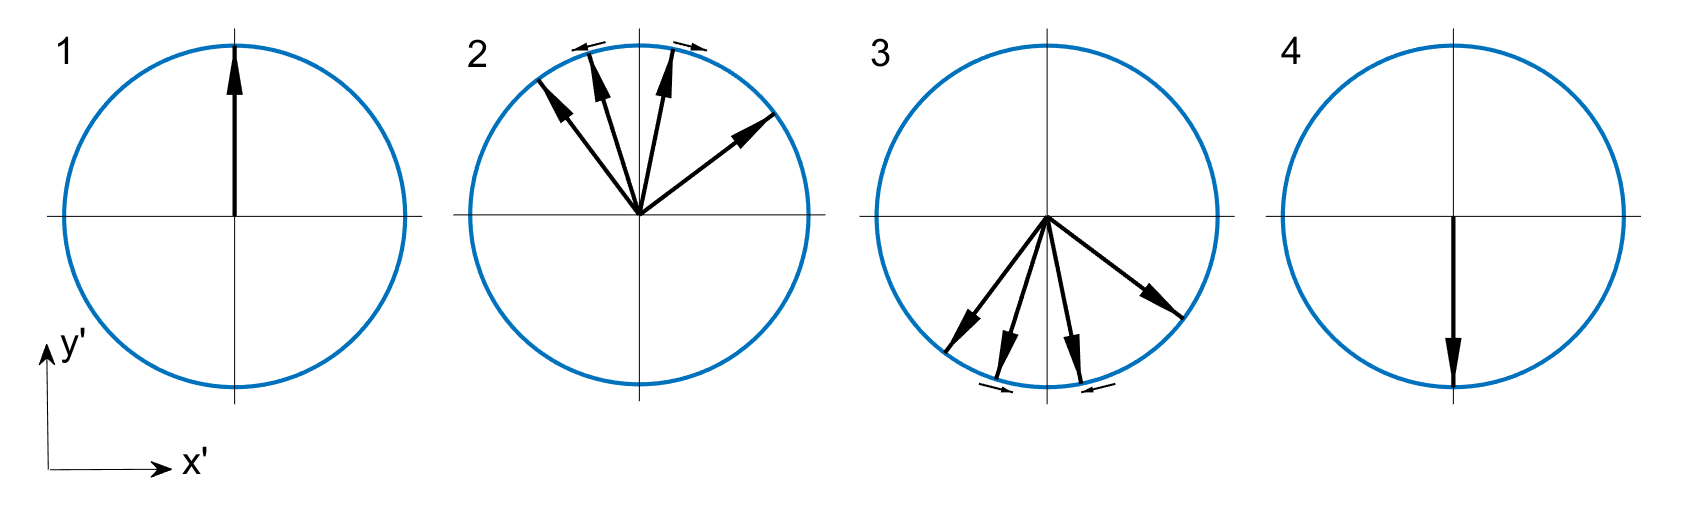
\includegraphics[width = \textwidth]{figures/background/spinecho_evolution.eps}
		\caption{}
		\label{fig:spinecho_evolution}
	\end{subfigure}

	\caption[The spin echo sequence and the evolution of spin under a spin echo sequence.]{a) Spin echo sequence and (b) an indication of the evolution of spins under a spin echo sequence. This shows how the 180\degree\ refocusing pulse acts to refocus the spins after a time $\mathrm{TE}$.}
	\label{fig:spinecho}
\end{figure}
It is possible to undo the effects of $\mathrm{T}_2'$ by designing a pulse sequence to `refocus' the spins, forming what is known as a spin echo.
%Spin echo sequences also enable localisation by combining \ac{RF} pulses with magnetic field gradients.
The first spin echo sequence was introduced by Edwin Hahn in 1950 \cite{Hahn1950}. The simplest sequence to form a spin echo consists of a 90\degree\ pulse to excite the spins followed by a 180\degree\ pulse after a delay. 
This sequence is shown in the diagram in \Cref{fig:spinecho} along with how the signal varies during the pulse sequence.
 
\Cref{fig:spinecho_evolution} represents how the magnetisation evolves through the pulse sequence with the four diagrams corresponding to the points marked in \Cref{fig:spinechosequence}. 
At point 1, immediately following the 90\degree\ pulse, all the magnetisation has been flipped into the transverse plane and is in phase - meaning all the magnetic moments of the spins point in the same direction in the x-y plane. 

The field inhomogeneities cause the different spins to feel slightly different magnetic fields and so precess at slightly different frequencies. 
This causes the spins to lose phase-coherence as indicated at point 2, and so the signal decays with $\mathrm{T}_2^*$.  

At point 3, following the 180\degree\ pulse, the spins remain out of phase with one another, but the 180\degree\ pulse has flipped their orientations across the $x'$-axis. 
The magnetic field the spins feel is still the same, so despite their flip in orientation, they still precess in the same direction. 
This means that the evolution that caused the spins to dephase begins to rewind and bring the spins back into phase coherence. 
After a time equal to the time between the 90\degree\ and 180\degree\ pulses, at point 4, the spins will be brought completely back in phase - or, refocused - and the spin echo is formed. 

The signal at point 4 will still be lower in magnitude than that at point 1 since the $\mathrm{T}_2$ relaxation will still occur as it is an inherent property of the matter. 
The spin echo does, however, refocus the $\mathbf{B}_0$ inhomogeneities. 
The time between the 90\degree\ pulse and the formation of the echo is known as the \ac{TE}. 

The spin echo sequence shown in \Cref{fig:spinecho} forms the basis of the standard \ac{PGSE} diffusion MRI sequence which is introduced in the following section, along with a description of the physics behind diffusion MRI. 

\section{Diffusion MRI}
\label{sec:diffusion_physics}
Diffusion MRI (dMRI) sensitises the \ac{MRI} signal to the motion of water molecules due to diffusion. The following section describes the physics behind diffusion and how the diffusion impacts the \ac{MRI} signal.

% Diffusion MRI simulations attempt to synthesise dMRI signals through models of our understanding of the underlying diffusion processes.
% These simulations broadly fall into two categories: solutions of the diffusion equation and Monte-Carlo simulations of the diffusion dynamics.

% The diffusion equation relates the rate of change of concentration to the spatial variation in concentration according to
% \begin{equation}
%   \frac{\partial c(\vec{r}, t)}{\partial t} = D\nabla^2 c(\vec{r}, t)\,.
% \end{equation}
%Diffusion \ac{MRI} simulations are ultimately trying to synthesise the \ac{dMRI} signal through models of our understanding of the underlying diffusion processes.
%This section briefly covers the physics that gives rise to the \ac{dMRI} signal. 

The diffusion process is driven by the Brownian motion of particles in fluids.
The thermal kinetic energy of particles causes them to move around rapidly, however particles frequently collide with each other (for instance, molecules in water at room temperature experience around 60 billion collisions per second \cite{Denny1993}) creating a very tortuous, random path.

Diffusion \ac{MRI} sensitises the MR signal to this motion by exploiting the dephasing of spins as a result of magnetic field gradients.


The magnetic field will generally have a uniform component from the main $B_0$ field, and spatially and/or time varying components due to deliberate magnetic field gradients or typically unwanted effects such as magnetic susceptibility inhomogeneities and concomitant fields \cite{Haacke1999}. In general, $B(\mathbf{r}, t)$, the magnitude of the magnitude of the magnetic field at a position $\mathbf{r}$ at time $t$ is given by
\begin{equation}
  B(\mathbf{r}, t) = |\mathbf{B}| = |B_0\mathbf{\hat{z}} + \mathbf{\Delta B}(\mathbf{r}, t)|\,,
  \label{eq:mod_B}
\end{equation}
where $\mathbf{\Delta B}(\mathbf{r}, t)$ accounts for all of the variation in the magnetic field away from $B_0$. Note that $\mathbf{\Delta B}(\mathbf{r}, t)$ is a vector quantity which may have components in the $\mathbf{\hat{x}}$ and $\mathbf{\hat{y}}$ directions. 

An idealised expression for $\mathbf{\Delta B}(\mathbf{r}, t)$ often applied to \ac{MRI} assumes that all of the change in the magnetic field is due to an applied magnetic field gradient, $\mathbf{g}(\mathbf{r}, t)$, which only has a significant $\mathbf{\hat{z}}$ component. This means that \Cref{eq:mod_B} can be written as
\begin{align}
  B(\mathbf{r}, t) &= \left|B_0\mathbf{\hat{z}} + \left(\mathbf{g}(\mathbf{r}, t)\cdot\mathbf{r}\right) \mathbf{\hat{z}}\right|\,,\nonumber \\
                      &= B_0 + \mathbf{g}(\mathbf{r}, t)\cdot\mathbf{r}\,.
                        \label{eq:mod_B_ideal}
\end{align}

Magnetic field gradients introduce a deliberate variation in the magnetic field which, according to \Cref{eq:LarmorFreq}, causes the Larmor frequency to vary spatially as well temporally.

Since the Larmor frequency varies spatially, spins in different locations will precess at different frequencies and accrue a phase shift relative to spins in different locations. 
The incremental phase, $d\phi$, accrued for a single spin, $i$, in an infinitesimal time, $dt$, % assuming a gradient in the $z$ direction
is given by
\begin{equation}
  % \phi(t, \mathbf{g}(\mathbf{r}(t), t)) = \gamma B_0 t + \gamma \int_0^t \mathbf{g}(\mathbf{r}(t'), t')\cdot\mathbf{r}(t')dt'\,,
  % \label{eq:phase_singlespin}
  d\phi_i = \gamma B(\mathbf{R}_i(t), t) dt\,,
  \label{eq:dphi}
\end{equation}
% where $\gamma$ is the gyromagnetic ratio, $B_0$ is the main field strength, $\mathbf{r}(t')$ is the position of the particle and $\mathbf{g}(\mathbf{r}(t'), t')$ is the (potentially spatially varying and time-dependent) magnetic field gradient.
where $\gamma$ is the gyromagnetic ratio and  $\mathbf{R}_i(t)$ is the position of the particle at time $t$. %and $B(\mathbf{r}(t), t)$ is the magnitude of the magnetic field at position $\mathbf{r}(t)$ and time $t$.

Putting \Cref{eq:mod_B_ideal} into \Cref{eq:dphi} and integrating over the time of the diffusion experiment will give the total phase accrued for a single spin:
\begin{equation}
  % \phi(t, \mathbf{g}(\mathbf{R}_i(t), t)) = \gamma B_0 t + \gamma \int_0^t \mathbf{g}(\mathbf{R}_i(t'), t')\cdot\mathbf{R}_i(t')dt'\,,
  \phi(\mathbf{R}_i(t)) = \gamma B_0t + \gamma\int_0^t\mathbf{g}(\mathbf{R}_i(t'), t')\cdot\mathbf{R}_i(t')dt'\,,
  \label{eq:phase_singlespin}
\end{equation}


The first term in this equation is the phase accrued due to the main magnetic field which will be the same for all spins in the system.
The second term is the phased accrued due to the gradient, which will be dependent on the motion of each individual spin.
The dot product here indicates that only displacement projected onto the gradient direction affects the phase, allowing the gradient direction to be used to probe the diffusion in different directions.

\begin{figure}
  \centering
  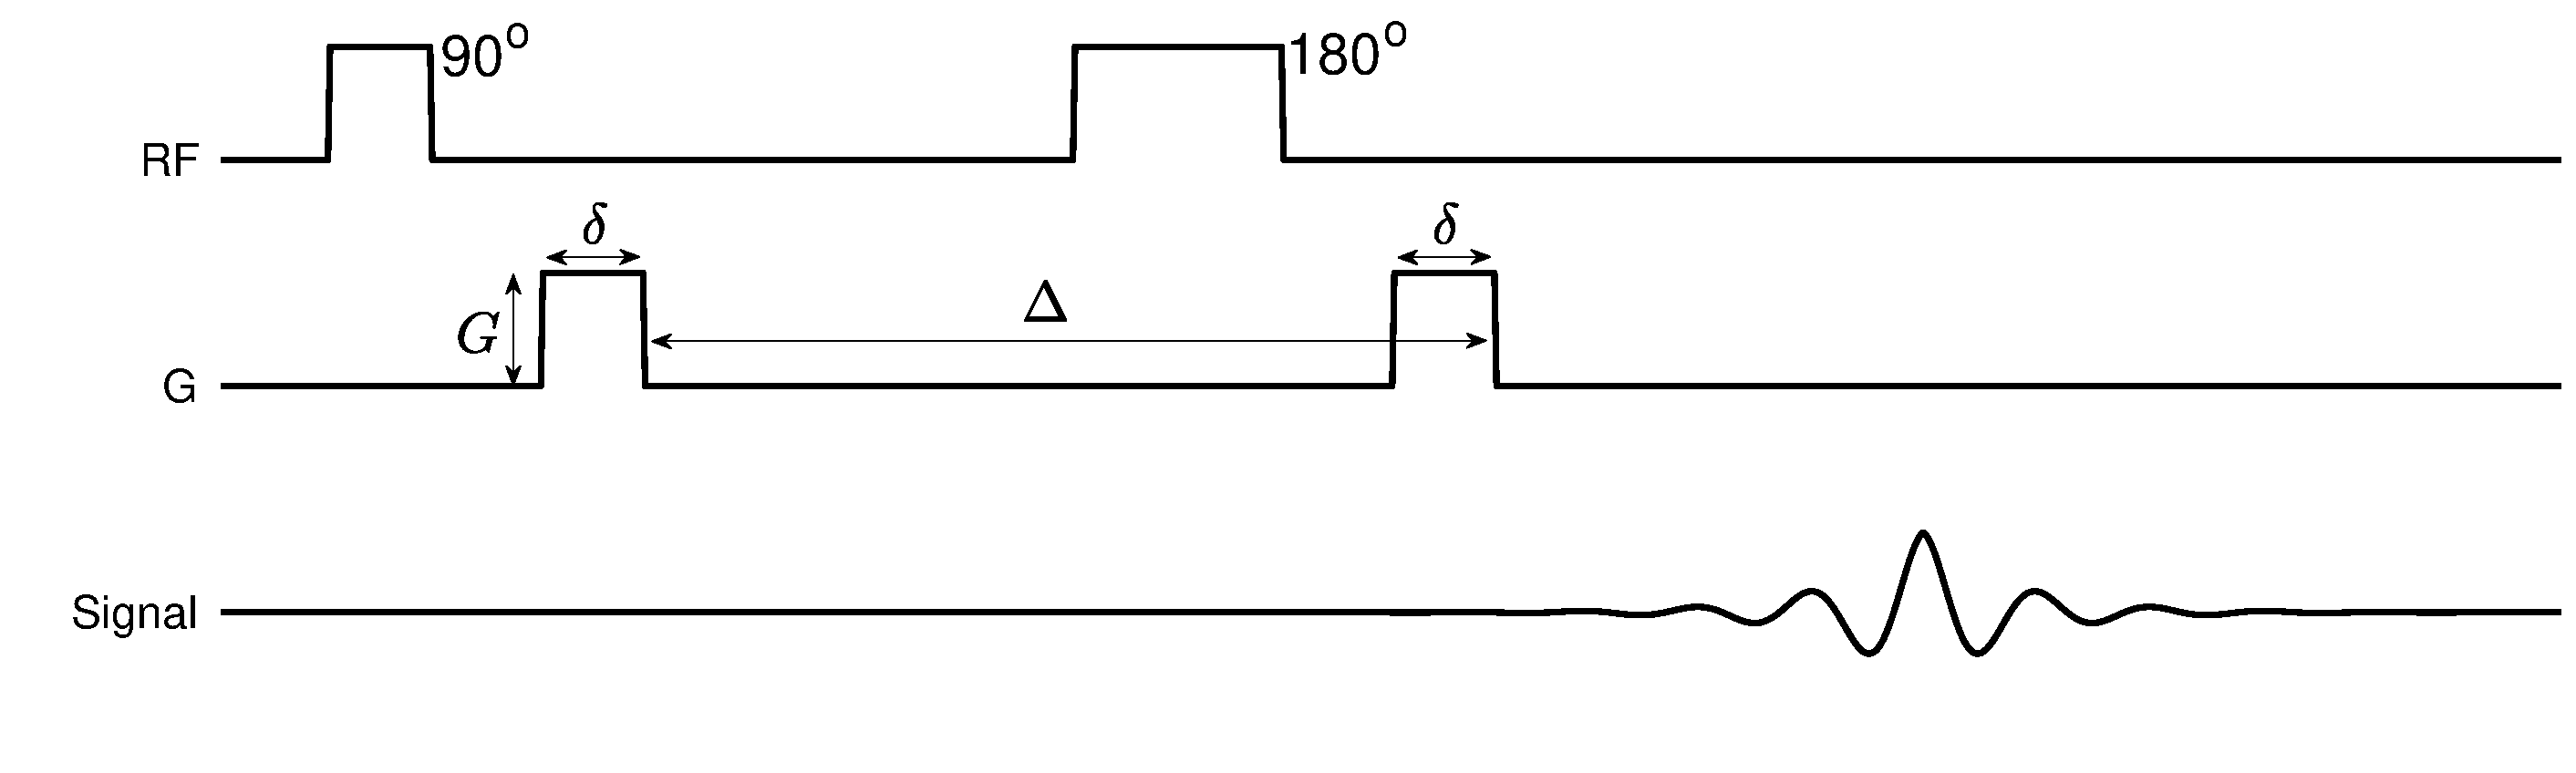
\includegraphics[width=0.9\textwidth]{figures/background/PGSE_diagram.eps}
  \caption{The standard \acl{PGSE} sequence used in \ac{dMRI}.}
  \label{fig:PGSE_diagram}
\end{figure}

The first diffusion MR sequence, introduced by Stejskal and Tanner in 1965\cite{Stejskal1965}, is the \acf{PGSE} sequence, shown in \Cref{fig:PGSE_diagram}.
The PGSE sequence consists of a standard spin echo sequence with a pair of gradient pulses added either side of the refocussing pulse.
In the ideal case, each pulse is rectangular with a gradient strength, $G$, and duration, $\delta$ and they are separated by a time, $\Delta$.  

The effect of this pulse sequence can be simplified by considering the case when $\delta \ll \Delta$. This is known as the \ac{SGP} approximation and means that the motion of spins during the pulses can be ignored. 

Under the \ac{SGP} approximation, the phase accrued by a spin at a position $\mathbf{R}_0$ during a pulse at a time $t_0$ will be
\begin{equation}
  \phi(\mathbf{R}_0) = \gamma B_0\delta +  \gamma \delta \mathbf{g(R_0)}\cdot\mathbf{R_0}\,.
  \label{eq:phi_single_SGP}
\end{equation}
Here, $\mathbf{R}_0$ refers to the spin position at time $t=t_0$ and is not time-dependent, because under the SGP approximation the motion of spins during the pulse is assumed to be negligible. 

The 180\degree\ pulse in the \ac{PGSE} sequence is crucial, since it flips the orientation of the spins' magnetic moments as in the spin echo sequence in \Cref{fig:spinecho}.
Not only does this refocus $\mathrm{T}_2^*$ effects as outlined in \Cref{sec:spin_echoes}, but similarly, it means that the phase accrued due to the first gradient pulse now has a negative sign relative to the phase that will be accrued due to the second pulse. %due to the second gradient pulse has opposite sign to the phase accrued due to the first pulse. 

A spin which is at a position $\mathbf{R}_0$ during the first pulse and then diffuses to a position $\mathbf{R}_1$ during the second pulse will therefore have a relative phase shift of 
\begin{equation}
  \Delta\phi(\mathbf{R}_1 - \mathbf{R}_0) = \gamma\delta\mathbf{g} \cdot \left(\mathbf{R}_1 - \mathbf{R}_0\right)\,.
  \label{eq:delta_phi}
\end{equation}

The $B_0$ term from \Cref{eq:phi_single_SGP} is the same for both gradient pulses, meaning that during the subtraction in \Cref{eq:delta_phi} it cancels and the only relative phase shift comes from the diffusive motion.

The total MR signal comes from an ensemble of spins, each with their own random Brownian motion and thus, from \Cref{eq:delta_phi}, their own relative phase shift.
To get to the total MR signal, we need to consider the probability that a particle starts at position $\mathbf{R}_0$ (i.e. the initial spin density, $\rho(\mathbf{R}_0)$, which can generally be considered uniform within a voxel \cite{Price1997}) and the probability that a particle which starts at $\mathbf{R}_0$ moves to $\mathbf{R}_1$ during the time $\Delta$, $P(\mathbf{R}_0, \mathbf{R}_1, \Delta)$.
Putting these together, gives an expression for the total MR signal\cite{Price1997,Stejskal1965}:
\begin{equation}
  S(\mathbf{g}, \Delta) = S(\mathbf{0}, \Delta)\int\int \rho(\mathbf{R}_0)P(\mathbf{R}_0, \mathbf{R}_1, \Delta) e^{i\gamma\delta\mathbf{g} \cdot (\mathbf{R}_1 - \mathbf{R}_0)}  d\mathbf{R}_0d\mathbf{R}_1\,.
  \label{eq:total_signal_sgp}
\end{equation}

This quantity, $P(\mathbf{R}_0, \mathbf{R}_1, \Delta)$, is known as the diffusion propagator and is of great interest for diffusion MRI because $P(\mathbf{R}_0, \mathbf{R}_1, \Delta)$ encodes the information about the environment in which the spins are diffusing. 
For diffusion in an isotropic, homogeneous medium, the diffusion propagator is a Gaussian distribution \cite{Price1997}:
\begin{equation}
  P(\mathbf{R}_0, \mathbf{R}_1, t) = \left(4\pi Dt\right)^{-\sfrac{3}{2}}\exp\left(-\frac{(\mathbf{R}_1 - \mathbf{R}_0)^2}{4Dt}\right)\,.
  \label{eq:propagator_diffusion}
\end{equation}

In the case of Gaussian diffusion, \Cref{eq:total_signal_sgp} can be solved analytically and will give an MR signal attenuation (that is, $S(t)/S(0)$) which is also Gaussian\cite{Stejskal1965,Price1997}
\begin{equation}
  E(g, \Delta) = \exp(-\gamma^2g^2\delta^2D\Delta)\,.
  \label{eq:sgp_signal_gaussian}
\end{equation}

The general form of this expression, accounting for finite duration gradient pulses, can also be analytically derived to give the Stejskal-Tanner equation \cite{Stejskal1965,Kuchel2012}
\begin{align}
  \ln(E) &= -\gamma^2g^2\delta^2D(\Delta - \delta/3)\,,\label{eq:stejskal_tanner}\\
  &= -bD\,,
\end{align}
where $b = \gamma^2g^2\delta^2(\Delta - \delta/3)$ is the so-called $b$-value which describes the strength of the diffusion encoding. 

We can formulate a more general form of  \Cref{eq:total_signal_sgp} without requiring any assumptions on the gradients (such as the \ac{SGP} approximation used above) as \cite{Price1997,Hall2009}
\begin{equation}
  S(\mathbf{g}, t) = S(\mathbf{0}, t) \int_{-\infty}^{\infty} P(\phi, t) e^{i\phi} d\phi\,,
  \label{eq:sig_phi_complex}
\end{equation}
where the phase, $\phi$ will be given by \Cref{eq:phase_singlespin} and $P(\phi, t)$ is the probability density function of the phase distribution after a time $t$.

In the case of restricted diffusion (i.e.\ diffusion in an inhomogeneous or anisotropic environment) the form of the diffusion propagator becomes more complex and closed form solutions of \Cref{eq:total_signal_sgp,eq:sig_phi_complex} are only possible for certain simple geometries and assumptions.

Analytical solutions can be found for some simple restricting geometries such as spheres, cylinders and parallel plates \cite{Neuman1974, Balinov1993,Callaghan1995}.
For more complex environments, however, an analytical solution is intractable and we must rely on simulations to approximate the \acl{dMRI} signal.  

\begin{comment}
The total MR signal comes from an ensemble of spins, each with their own random Brownian motion and thus, from  \Cref{eq:phase_singlespin}, their own phase. This gives the total \ac{dMRI} signal, $S(t, \mathbf{g})$ as

where $S(t, \mathbf{0})$ is the signal with no gradients applied. $P(\phi, t)$ is the probability density function of the phase distribution after a time $t$.

From \Cref{eq:phase_singlespin}, we see that the individual phases, and thus the phase distribution, depend on the motion of the particles as well as the description of the diffusion sensitising gradient (in the case of standard pulsed gradient experiment that is the timing, strength, duration and orientation of the gradient) \cite{Price1997}.

This quantity, $P(\phi, t)$, is closely related to another property of great interest for diffusion MRI known as the diffusion propagator, $P(\mathbf{R}_0, \mathbf{R}_1, t)$. $P(\mathbf{R}_0, \mathbf{R}_1, t)$ is the probability that a particle initially at a position $\mathbf{R}_0$ moves to $\mathbf{R}_1$ in a time $t$.
For diffusion in an isotropic, homogeneous medium, the diffusion propagator is a Gaussian distribution \cite{Price1997}:
\begin{equation}
  P(\mathbf{R}_0, \mathbf{R}_1, t) = \left(4\pi Dt\right)^{-\sfrac{3}{2}}\exp\left(-\frac{(\mathbf{R}_1 - \mathbf{R}_0)^2}{4Dt}\right)\,.
  \label{eq:propagator_diffusion}
\end{equation}

\end{comment}

\subsection{The \acl{BT} Equations}
\label{sec:bg_bloch_torrey}
As well as describing the \ac{dMRI} signal by considering the microscopic diffusion of spins, a macroscopic formulation can be derived considering Fick's laws of diffusion. The combination of the Bloch equations (\Cref{eq:blochx,eq:blochy,eq:blochz}) with Fick's second law of diffusion leads to the \ac{BT} equations, proposed by H.\ C.\ Torrey in 1956\cite{Torrey1956,Callaghan1991,Price2009}:

\begin{equation}
  \frac{\partial\mathbf{M(r},t)}{\partial t} = \gamma \mathbf{M \times B(r}, t) - \frac{M_x\mathbf{\hat{x}} + M_y\mathbf{\hat{y}}}{\mathrm{T}_2} - \frac{(M_z - M_0)\mathbf{\hat{z}}}{\mathrm{T}_1} + \nabla \cdot \left(\mathbf{D} \nabla \mathbf{M}\right)\,.
  \label{eq:bloch_torrey}
\end{equation}

This version of the \ac{BT} equation is sometimes referred to as the standard \ac{BT} equation. An additional term can be added to account for the evolution of the magnetisation due to a flow, described by a velocity field $\mathbf{v}$ to get the generalised \ac{BT} equation \cite{Jeener2002,Beltrachini2016}. However, this flow term is often dropped, assuming no net flow, in the application to \ac{dMRI}, leaving \Cref{eq:bloch_torrey}. 
$\mathbf{D}$ is the diffusion tensor, a generalisation of the diffusion coefficient, $D$, to allow for anisotropic diffusion. In short, this means that diffusion happens at a different rate in different directions.
It is the $\mathbf{D}$ term in \Cref{eq:bloch_torrey} which encodes the evolution of the magnetisation when there is diffusion.

In general, the \ac{BT} equations cannot be solved analytically, apart from in some simple cases such as isotropic free diffusion.
For instance, the solution to the \ac{BT} equations in isotropic free diffusion can be shown to give the expected Stejskal-Tanner equation, \Cref{eq:stejskal_tanner} \cite{Price1997}.

For complex geometries, as with the case above, we must rely on computational methods to come to a solution for the \ac{BT} equations. 



\section{Diffusion Simulation}
\label{sec:diffusion_simulation}
Diffusion simulations attempt to evaluate \Cref{eq:sig_phi_complex} or \Cref{eq:bloch_torrey} computationally. Simulation approaches broadly fall into two categories: numerical solutions of the \ac{BT} equation and \ac{MC} simulations of the diffusion dynamics. This section introduces these techniques, highlighting the some of the similarities and differences between them. 


At a high level, all diffusion simulations have three common components: the substrate, the diffusion dynamics and the measurement.
The substrate describes the environment in which the diffusion is taking place. A common example of this is parallel cylinders representing axons in white matter.
The diffusion dynamics describe our understanding of the processes underlying the diffusive motion of molecules and the measurement describes how this diffusive motion results in a synthetic \ac{dMRI} signal.
\subsection{Numerical Solutions}
\label{sec:numerical_solutions}
Numerical solution approaches generally attempt to solve the \acl{BT} equation \cite{Torrey1956}.
These approaches combine both the dynamics and the measurement components of the diffusion simulation by solving for the magnetisation in  \Cref{eq:bloch_torrey}.
The third component, the substrate, defines boundary conditions required for the solution of the equation. 

There are two typical methods for solving the \ac{PDE} in \Cref{eq:bloch_torrey}, \acp{FDM} and \acp{FEM}.
Finite difference methods evaluate the \ac{PDE} using a local Taylor expansion at discrete points which are generally uniformly separated in each spatial as well as the temporal dimension \cite{Grossmann2007}.
\acp{FDM} are an efficient method for solving \acp{PDE} when the problem can fit into a rectangular grid, however they are less effective when applied to complex geometries \cite{Hagslatt2003, Grossmann2007}.

Finite element methods subdivide the domain into small elements which are simple geometric shapes, though unlike the \acp{FDM}, they do not have to form a regular grid, but rather an arbitrary mesh.
In each element, the \ac{PDE} solution is approximated by simple functions such as a linear combination of polynomials.
The combination of all of these local approximations can be solved to give a numerical solution of the \ac{PDE} across the whole domain \cite{Logan2007}.
\acp{FEM} are generally more complex to formulate and implement than \acp{FDM}, however the added complexity can be worth the effort for more difficult problems in which \acp{FDM} may be ineffective \cite{Iserles2009}.

\subsection{Monte-Carlo Simulations}
\label{sec:montecarlo}
Monte-Carlo methods take a different approach to the simulation of the \ac{dMRI} signal. Monte-Carlo methods simulate the Brownian motion of a large number of particles, simulating the motion of each particle individually, along with the MR acquisition to generate the \ac{dMRI} signal.

There exist many different implementations of the Monte-Carlo simulation of \ac{dMRI} \cite{Yeh2013,Nilsson2012,Landman2010,Balls2009,Hall2009,Ford1997,Szafer1995}, however the underlying principles are similar for all of them. The following is a general description of the \ac{MC} simulation process, however the specifics for each different implementation may vary. 

% There are three main components of an MC diffusion simulation: (1) the environment in which particles are diffusing (often called the substrate), (2) the dynamics of the Brownian motion and (3) the MR pulse sequence used to acquire the signal. 


Most early \ac{MC} studies used simple, easily parametrised substrates like regularly packed cuboids \cite{Szafer1995} or cylinders \cite{Ford1997}.
As computational power has increased, so too has the capacity for more and more complex substrates.
This includes cylinders with randomly distributed radii \cite{Hall2009}, undulating  cylinders \cite{Nilsson2012}, beading cylinders \cite{Budde2010} and meshes, both generated from high resolution microscopy of tissue \cite{Panagiotaki2010} and computer generated cell models \cite{Palombo2019,Rafael-Patino2018}.

The Brownian motion of particles is typically simulated as a random walk of many independent particles. The time domain is discretised into many time points and at each time point each particle takes a random step through the substrate.  
One step of the random walk can be briefly summarised as shown in \Cref{alg:MC_random_walk}.
\begin{algorithm}
  \begin{algorithmic}
    \State generate randomly oriented step vector
    \State check if step crosses a barrier 
    \While{step crosses barrier}
    \State amend step according to barrier interaction (e.g. elastic reflection)
    \State repeat barrier checking on amended step
    \EndWhile
    \State update the particle position 
  \end{algorithmic}
  \caption{Basic algorithm for taking a step in the random walk.}
  \label{alg:MC_random_walk}
\end{algorithm}
 
Following the Brownian motion, each particle in the simulation will have taken many steps giving each particle a unique trajectory that it has traversed.
The incremental phase, $\Delta \phi$, accrued at each step can be calculated from a discrete version of \Cref{eq:phase_singlespin}. Under the assumption of uniform $B_0$, only the gradient term matters, giving
\begin{equation}
  \Delta \phi = \gamma \mathbf{g}(\mathbf{R}(t), t) \cdot \mathbf{R}(t)\, \Delta t \,,
  \label{eq:deltaPhi}
\end{equation}
where $\Delta t$ is the duration of the step and $\mathbf{g}(\mathbf{R}(t), t)$ and $\mathbf{R}(t)$ are the gradient and particle position during that step respectively.

The phase accumulation in \Cref{eq:deltaPhi} for each spin in the simulation can be combined with \Cref{eq:sig_phi_complex} to approximate the total signal for the \ac{dMRI} acquisition as
\begin{equation}
  S = \sum_j e^{i\Phi_j}\,,
  \label{eq:MCsignal}
\end{equation}
where $\Phi_j$ is the total phase accrued for each spin. 

Monte-Carlo simulations are a powerful tool for \ac{dMRI} simulation due to their ability to handle any arbitrary substrate and MR pulse sequence.
Additionally, \ac{MC} simulations can be modified to account for effects that are more difficult to formulate for analytical and numerical solutions of the diffusion equation such as semi-permeable membranes, membrane-particle interactions and spatially and/or temporally varying $\mathrm{T_1, T_2}$ and diffusivities.

A drawback of \ac{MC} simulation, particularly for complex substrates is the need to simulate enough spins to mimic the ensemble behaviour of spins \emph{in vivo} as well as enough discrete time points to adequately capture the dynamics through the pulse sequence.
The huge number of calculations required to handle large simulations can be alleviated by exploiting the inherent parallel nature of the problem to run simulations in parallel on a \ac{CPU} cluster or, even more effectively, a GPU cluster.

\section{Neural growth}
\label{sec:bg_nerual_growth}
Neural development is a complex and constantly evolving field of research, due in part to the sheer size and complexity of the fully developed brain - for instance, during human development about 100 billion cells are generated with about 100 trillion connections between them \cite{Price2017}. This means that development on an individual neuron basis can only be studied in simple organisms with only a few hundred neurons and even then there are many mechanisms which are yet to be fully understood \cite{Price2017}.

In spite of this, many neural growth mechanisms have been identified and studied in simple organisms and \emph{in vitro} experiments \cite{Price2017,Rauch2013,Nikic2011,Dent2011,Polleux2010,Lowery2009,Mortimer2008,Sakisaka2005,Scott2001,NAP1785} which give us some understanding of how neurons take their shape.

At this point, a brief review of some biological terms that will be used extensively is useful. Firstly, brain cells can typically be split into two categories: neurons and glial cells. Neurons are the cells which transmit and receive signals within the brain and between the brain and the rest of the body. Neuronal cells can be thought of in a few parts, firstly the cell body, or soma, contains the nucleus of the cells, secondly long extensions known as neurites grow out from the soma. Neurites themselves are broken down into either dendrites or axons. A neuron typically has a single axon which is a long neurite which carries information away from the soma while the dendrites form a branched tree which integrates incoming information to the neuron \cite{Price2017}. Glial cells perform many functions which enable the nervous system to function efficiently such as creating the myelin sheaths which cover the axons to facilitate fast and efficient transmission of signals.

On a higher level, the brain can broadly be split into two types of tissue, \acf{WM} and \acf{GM}. Grey matter contains the majority of the neuronal cell bodies in the brain while the \acl{WM} is typically composed of primarily axons connecting different \ac{GM} regions together. It is the \acl{WM} which is of interest for this work, so it is important to understand how axons grow to understand how the \ac{WM} is organised.

\subsection{Axonal growth mechanisms}
\label{sec:bg_axonal_growth}



%%% Local Variables:
%%% mode: latex
%%% TeX-master: "../main"
%%% End:
